\documentclass{fisatprojectfinal}
\usepackage{listings}

\title{Pose Estimation Using Deep Learning}
\team{Aman K. Shihab \\ Aneeta Shajan}
\author{Aman K. Shihab}
\regno{FIT19CS015}
\begin{document}
\maketitle
\makecert

\newpage
\pagenumbering{roman}
\setcounter{page}{1}
\newgeometry{top=4cm,bottom=0.1cm}
\thispagestyle{plain}
\renewcommand\abstractname{ABSTRACT}
\begin{abstract}
\vspace{5cm}
Single-person human pose estimation facilitates markerless movement analysis in sports, as well as in clinical applications.
Still, state-of-the-art models for human pose estimation generally do not meet the requirements of real-life applications.
The proliferation of deep learning techniques has resulted in the development of many advanced approaches. However,
with the progresses in the field, more complex and inefficient models have also been introduced, which have caused
tremendous increases in computational demands. To cope with these complexity and inefficiency challenges, we propose
a novel convolutional neural network architecture, called EfficientPose, which exploits recently proposed EfficientNets
in order to deliver efficient and scalable single-person pose estimation. EfficientPose is a family of models harnessing
an effective multi-scale feature extractor and computationally efficient detection blocks using mobile inverted bottleneck
convolutions, while at the same time ensuring that the precision of the pose configurations is still improved. Due to its low
complexity and efficiency, EfficientPose enables real-world applications on edge devices by limiting the memory footprint
and computational cost. The results from our experiments, using the challenging MPII single-person benchmark, show that
the proposed EfficientPose models substantially outperform the widely-used OpenPose model both in terms of accuracy and
computational efficiency. In particular, our top-performing model achieves state-of-the-art accuracy on single-person MPII,
with low-complexity ConvNets.
\end{abstract}



\newpage
\renewcommand\abstractname{Contribution by Author}
\thispagestyle{plain}
\begin{abstract}
\vspace{5cm}
The model was fine-tuned using the Leeds Sports dataset. We observed some points increase in accuracy of the model.
Work is progressing currently on obtaining dataset to finetune it for Physiotherapy pose detection and correction.
\vspace{1cm}
\begin{flushright}
Student Name
\end{flushright}
\end{abstract}

\newpage
\renewcommand\abstractname{ACKNOWLEDGEMENT}
\thispagestyle{plain}
\begin{abstract}
\vspace{5cm}
It gives me a great sense of pleasure to present the report of the project work undertaken during BTech 
semseter 6. I owe a special debt of gratitude to my Project Mentor \textbf{Mr. Pankaj Kumar G} for guiding and supporting us
throughout the course of this project. It's only due to his trust and support we were able to complete this project succesffully. I would also like to acknowledge
\textbf{Cognitive Computing Research Centre (CCRC) FISAT} for providing us with an environment and the experience to conduct research projects.
\par
I would like to extend my gratitude to out project co-ordinators \textbf{Ms. Chethna Joy} and \textbf{Ms. Remya R} for helping us in 
keeping the course of our project in track providing with appropriate ideas and information which were useful suring the duration of our project work.
\par
Finally, my deepest thanks to \textbf{Computer Science and Engineering Deptartment, Fisat} and our HOD \textbf{Dr. Jyothish K. John} for provinding us with the
correct environment and opprotunities to learn and grow. I would like to thank our University, for including this project as a part of the degree program.
\vspace{1cm}
\begin{flushright}
Aman K. Shihab
\end{flushright}
\end{abstract}
\newpage

\restoregeometry
\tableofcontents
\thispagestyle{plain}
\newpage

\cleardoublepage
\addcontentsline{toc}{chapter}{\listfigurename}
\listoffigures
\newpage

\cleardoublepage
\addcontentsline{toc}{chapter}{\listtablename}
\listoftables
\newpage



\chapter{Introduction}
\pagenumbering{arabic}
\setcounter{page}{1}
\renewcommand{\baselinestretch}{1.50}
\section{Overview}
Single-person human pose estimation (HPE) refers to the
computer vision task of localizing human skeletal keypoints
of a person from an image or video frames. Single-
person HPE has many real-world applications, ranging from
outdoor activity recognition and computer animation to clinical assessments of motor repertoire and skill practice
among professional athletes. The proliferation of deep
convolutional neural networks (ConvNets) has advanced
HPE and further widen its application areas. ConvNet-based
HPE with its increasingly complex network structures,
combined with transfer learning, is a very challenging task.
However, the availability of high-performing ImageNet
backbones, together with large tailor-made datasets, such
as MPII for 2D pose estimation, has facilitated the
development of new improved methods to address the
challenges.
\begin{figure}[h!]
\begin{center}
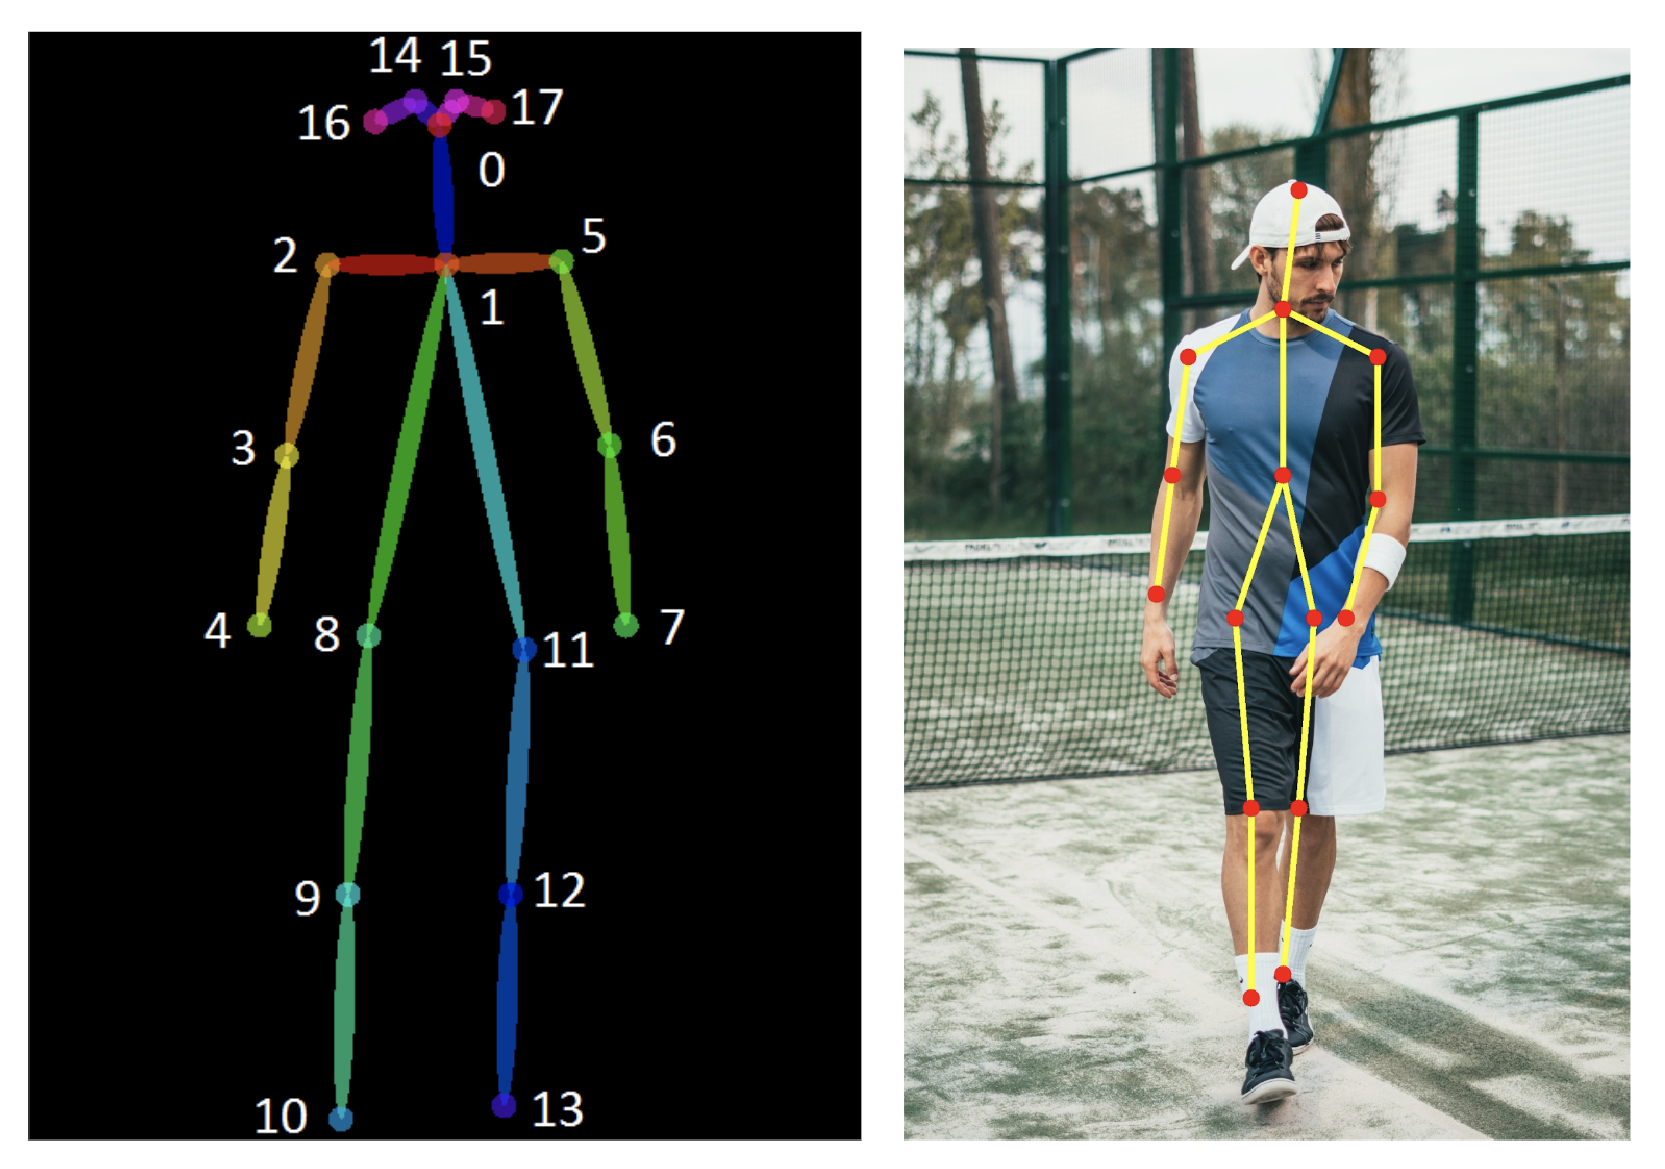
\includegraphics[scale=.3]{pose-estimation}
\caption{Human Pose Estimation Demo}
\end{center}
\end{figure}
An increasing trend in computer vision has driven towards
more efficient models. Recently, Efficient-
Net was released as a scalable ConvNet architecture,
setting benchmark record on ImageNet with a more com-
putationally efficient architecture. 
\section{Problem Statement}

Despite the availability of more performant, efficient layers and architecture's, it has not quite transalated
into fruitful results within human pose estimation, there is still a lack of architectures that
are both accurate and computationally efficient at the same
time. In general, current state-of-the-art architectures are
computationally expensive and highly complex, thus making them hard to replicate, cumbersome to optimize, and
impractical to embed into real-world applications. \par

Minimal and efficient model architectures are coveted for their ability to run on edge devices with minimal hardware requirements.
This also greatly reduces the response times thereby becoming increasingly relevant for real-time applications.
The ability to run real-time is a crucial feature for pose estimation, because often times in most applications it's desirable to obtain the outputs instantly to judge the output.

\section{Objective}

Primary objective is to exploit recent advances in ConvNets and shed some light onto
an improved approach called EfficientPose. The main idea
is to modify OpenPose, a well-known pose estimation model into a family of scalable ConvNets
for high-precision and computationally efficient single-person
pose estimation from 2D images. 
Then we evaluate the EfficientPose model by comparing
it against the original OpenPose model on single-person
HPE. After that, we compare it against the current state-of-
the-art single-person HPE methods on the official MPII
challenge, focusing on accuracy as a function of the number
of parameters. EfficientPose models aim to
elicit high computational efficiency, while bridging the gap
in availability of high-precision HPE networks.

\chapter{Related works}

Ever since the increased adoption of ConvNets for HPE following the
success of DeepPose has set the path for accurate HPE.
Another breakthrough in HPE was provided by OpenPose. OpenPose comprises a multi-
stage architecture performing a series of detection passes.
Provided an input image of 368 × 368 pixels, OpenPose
utilizes an ImageNet pretrained VGG-19 backbone to
extract basic features. The features are
supplied to a DenseNet-inspired detection block
arranged as five dense blocks, each containing three 3×
3 convolutions with PReLU activations. The detection
blocks are stacked in a sequence. First, four passes of part affinity fields map the associations
between body keypoints. Subsequently, two detection
passes predict keypoint heatmaps to
obtain refined keypoint coordinate estimates. In terms of
level of detail in the keypoint coordinates, OpenPose is
restricted by its output resolution of 46 × 46 pixels.
The OpenPose architecture can be improved by recent
advancements in ConvNets, as follows: First, automated
network architecture search has found backbones that are more precise and efficient in image
classification than VGG and ResNets. Compound model scaling can
balance the image resolution, width (number of networkchannels), and depth (number of network layers). This
resulted in scalable convolutional neural networks, called
EfficientNets, with which the main goal was to provide
lightweight models with a sensible trade-off between model
complexity and accuracy across various computational
budgets. For each model variant EfficientNet, from the
most computationally efficient one being EfficientNet-B0
to the most accurate model, EfficientNet-B7.The total no. of FLOPS increases by a factor of 2, given by:
	
	$$
	(\alpha. \beta^2. \gamma ^ 2) ^ \phi
	$$
where $$ \alpha = 1.2 , \beta = 1.1, \gamma = 1.15 $$
They denote the coefficients for depth, width and resolution respectively.
% \begin{table}[h!]
% \begin{center}
% 	\caption{World Population Table} 
% \begin{tabular}{|c|c|c|c|}
	
% \hline Rank & Country & Population  & Percentage  \\ 
% \hline 1 & China & 1,347,350,000 & 19.24\% \\ 
% \hline 2 & India & 1,210,193,422  & 17.28\% \\ 
% \hline 3 & United States & 313,269,000 & 4.47\% \\ 
% \hline 
% \end{tabular}
% %\caption{World Population Table} 
% \end{center}
% \end{table}
\begin{figure}[h!]
	\begin{center}
	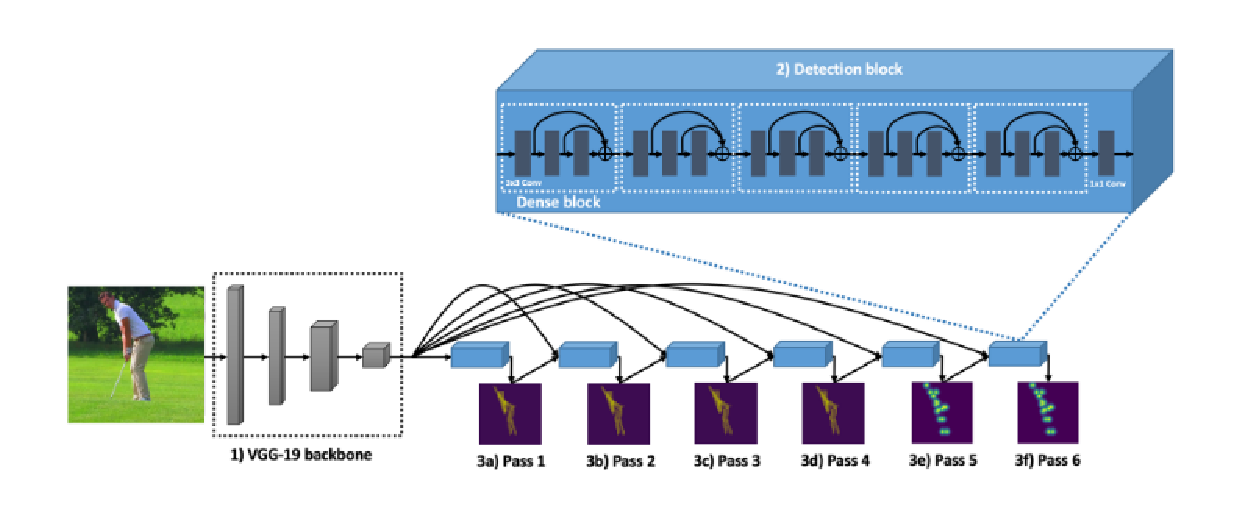
\includegraphics[scale=.8]{OpenPose}
	\caption{OpenPose}
	\end{center}
	\end{figure}
\par
Second, parallel multi-scale feature extraction has improved
the precision levels in HPE, emphasizing
both high spatial resolution and low-scale semantics.
However, existing multi-scale approaches in HPE are
computationally expensive, both due to their large size and
high computational requirements. For example, a typical
multi-scale HPE approach has often a size of 16 to 58
million parameters and requires 10 to 128 GFLOPS. To cope with this, we propose cross-
resolution features, operating on high- and low-resolution
input images, to integrate features from multiple abstraction
levels with low overhead in network complexity and with
high computational efficiency. Existing works on Siamese
ConvNets have been promising in utilizing parallel network
backbones. Third, mobile inverted bottleneck
convolution (MBConv) with built-in squeeze-and-
excitation (SE) and Swish activation integrated
in EfficientNets has proven more accurate in image
classification tasks than regular convolutions, while substantially reducing the computational costs. The efficiency of MBConv modules stem from
the depthwise convolutions operating in a channel-wise
manner. With this approach, it is possible to reduce the
computational cost by a factor proportional to the number
of channels. Hence, by replacing the regular 3 × 3
convolutions with up to 384 input channels in the detection
blocks of OpenPose with MBConvs, we can obtain more
computationally efficient detection blocks. Further, SE
selectively emphasizes discriminative image features,
which may reduce the required number of convolutions and
detection passes by providing a global perspective on the
estimation task at all times. Using MBConv with SE may
have the potential to decrease the number of dense blocks
in OpenPose. Fourth, transposed convolutions with bilinear
kernel scale up the low-resolution feature maps, thus
enabling a higher level of detail in the output confidence
maps.The main advantage
of this is that we can use ConvNets that are small and
computationally efficient enough to run on edge devices
with little memory and low processing power, which is
impossible with OpenPose. We can also alter the parameters of EfficientNet to obtain different variants
with accuracies and efficiencies that are different.


\chapter{Design}

\section{Introduction}
Here, the model architecture we use, namely EfficientPose exploits the recent advancements in ConvNets
and additionally concatenates high-level and low-level features. The net result is a much more efficient model
with better accuracy and needing fewer computaional resources.

\section{Architecture}

\begin{figure}[h!]
	\begin{center}
	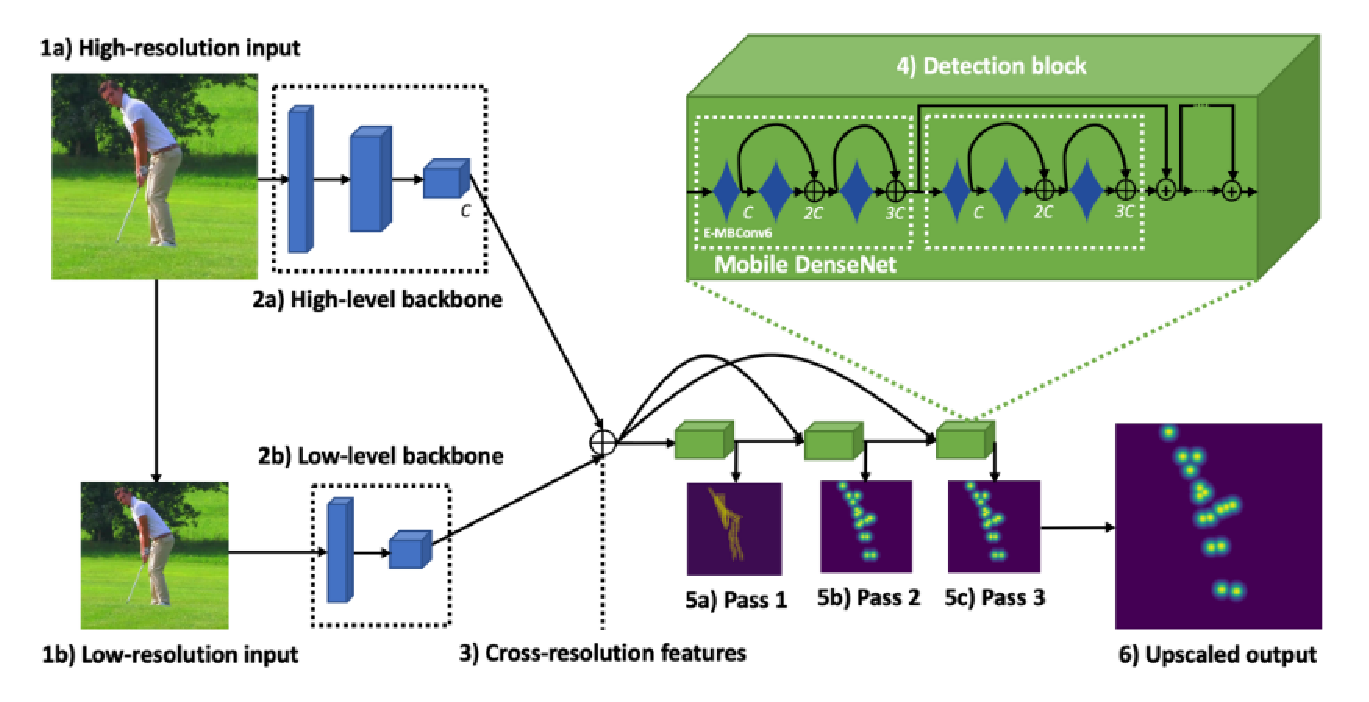
\includegraphics[scale=0.6]{EfficientPose}
	\caption{EfficientPose}
\end{center}
\end{figure}

The model takes in two inputs, one is the high-level features and second is the low-level features.
The low level features are obtained by downsampling an image to half of it's height and width using an average pooling layer.
The feature extractors here are initial layers of EfficientNet. For high level extractor, $\phi \in [0,7]$ and 
for the low level extractor $\phi \in [0,3]$.
\par
These extracted features and then concatendated together to obtain cross-resolution features.
This helps us to emphasize the important local factors in the image of interest.
\par
The input to the next phase of the model is the cross-resolution features obtained in the previous step.
Here the required keypoints are localized through an iterative process, where each
detection pass performs supervised prediction of output maps.
Each detection pass comprises a detection block
and a single 1 × 1 convolution for output prediction.
The detection blocks across all detection passes exhibit the
same basic architecture, comprising Mobile DenseNets.
Data from here is forwarded to the successive layers through skip connections.
Here, we also avoid downsampling of the output to preserve the resolution.
The original mobile convnets are modified by adding an E-swish activation function with $\beta$ value 1.25.
\par
The overall detection is performed in two rounds. Initially, the overall pose of the person is anticipated through a single pass of skeleton estimation. This helps especially when
there are multiple people present in the frame.
After the skeleton estimation is done two detection passes are performed to estimate heatmaps for points of interest.

\par
Another improvement on top of OpenPose is that, EfficientPose projects lower-resoltion image onto a higher resolution space using transposed convolution to allow an increased level of detail, whereas in OpenPose the heatmaps are
constrained to the lower space.
\section{Modules}
\subsection{EfficientNet}
In mathematics, Stirling's approximation (or Stirling's formula) is an approximation for large factorials. It is named after James Stirling.

\subsection{E-Swish}

\section{Accuracy Measures}
\chapter{Datasets}
\section{MPII Human Pose Dataset}
MPII Human Pose dataset is a state of the art benchmark for evaluation of articulated human pose estimation. The dataset includes around 25K images containing over 40K people with annotated body joints. The images were systematically collected using an established taxonomy of every day human activities. Overall the dataset covers 410 human activities and each image is provided with an activity label. Each image was extracted from a YouTube video and provided with preceding and following un-annotated frames. In addition, for the test set we obtained richer annotations including body part occlusions and 3D torso and head orientations.
The model was trained primarily on this dataset.

\section{Leeds Sports Dataset}
This dataset contains 2000 pose annotated images of mostly sports people gathered from Flickr using the tags shown above. The images have been scaled such that the most prominent person is roughly 150 pixels in length. Each image has been annotated with 14 joint locations. Left and right joints are consistently labelled from a person-centric viewpoint. Attributions and Flickr URLs for the original images can be found in the JPEG comment field of each image file. 
The ordering of the joints are as follows:
\begin{enumerate}
	\item Right Ankle
	\item Right Knew
	\item Right Hip
	\item Left Hip
	\item Left Knee
	\item Left Ankle
	\item Right Wrist
	\item Right Elbow
	\item Right Shoulder
	\item Left Shoulder
	\item Left Elbow
	\item Left Wrist
	\item Neck
	\item Head Top
\end{enumerate}
\chapter{Results}

\begin{figure}[h!]
	\begin{center}
	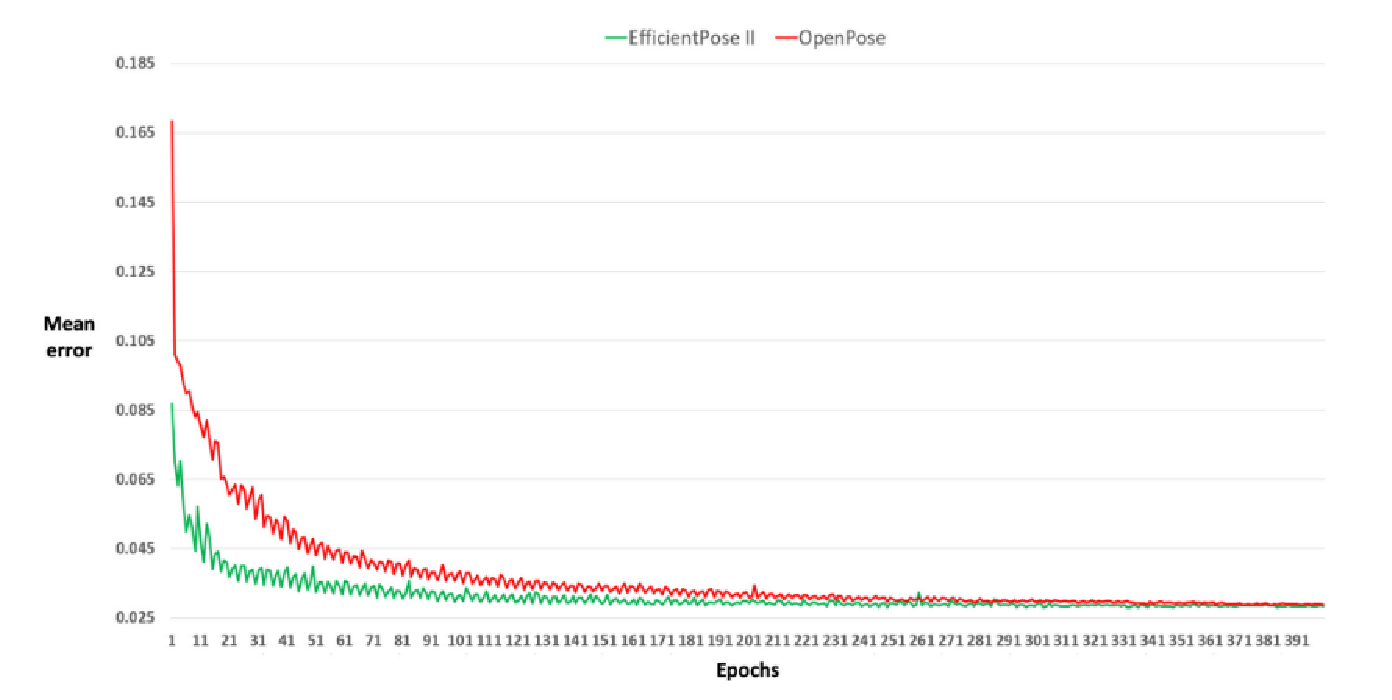
\includegraphics[scale=0.7]{TrainProgression}
	\caption{Convergence of mean error on OpenPose and EfficientPose}
\end{center}
\end{figure}
Some text

\begin{table}[h!]
	\begin{center}
		\caption{Comparison of EfficientPose and OpenPose on MPII validation dataset} 
	\begin{tabular}{|c|c|c|c|c|c|c|}
		
	\hline Model & Parameters & Parameter Reduction  & FLOPs  & FLOP Reduction & \(PCK_h\)@50 & \(PCK_h\)@10 \\ 
	\hline 1 & China & 1,347,350,000 & 19.24\% \\ 
	\hline 2 & India & 1,210,193,422  & 17.28\% \\ 
	\hline 3 & United States & 313,269,000 & 4.47\% \\ 
	\hline 
	\end{tabular}
	%\caption{World Population Table} 
	\end{center}
	\end{table}


\chapter{Outputs}

\begin{figure}[h!]
	\begin{center}
	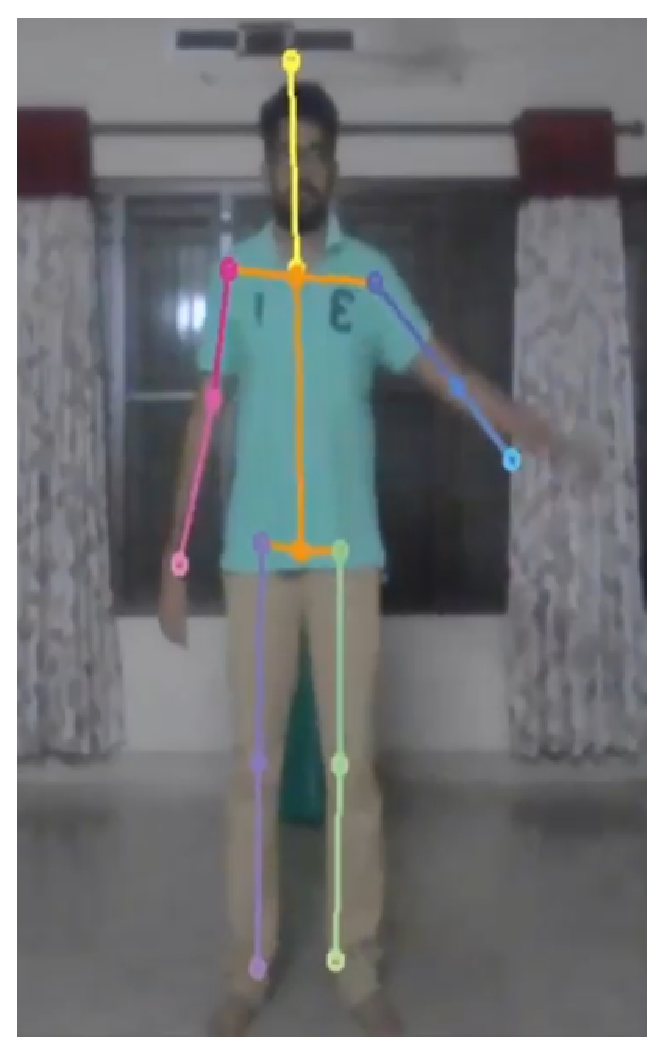
\includegraphics[scale=0.7]{op-1}
	\caption{Output 1}
\end{center}
\end{figure}

\begin{figure}[h!]
	\begin{center}
	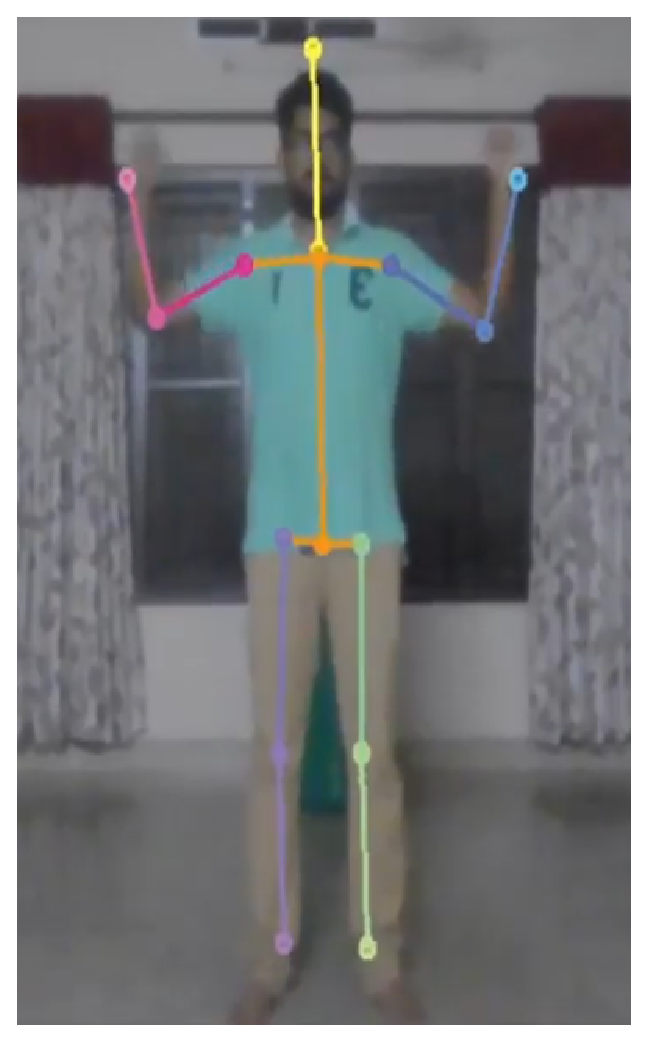
\includegraphics[scale=0.7]{pose-2}
	\caption{Output 2}
\end{center}
\end{figure}

\begin{figure}[h!]
	\begin{center}
	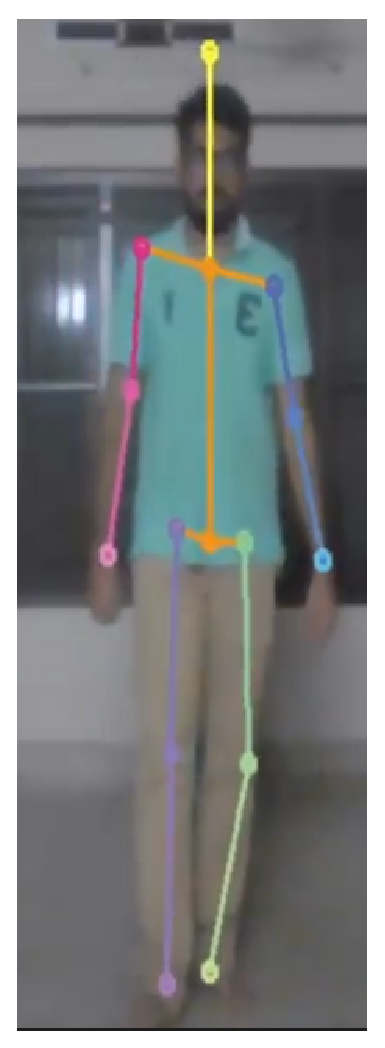
\includegraphics[scale=0.7]{pose-3}
	\caption{Output 3}
\end{center}
\end{figure}

\chapter{Conclusion}

By successfully exploiting the recent advances in convolutional neural networks, we have successfully made Single Person Pose-Estimation both more efficient and more accurate.
Due to this, many avenues of products in different fields may be developed that require real time pose estimation and hopefully it can be
used for wide ranging applications and products. The main advantage is the ability to run on edge devices which has been an achillies heal of
HPE for a long time.

\begin{thebibliography}{1}
\bibitem{Groos} EfficientPose: Scalable single-person pose estimation, ``Daniel Groos, Heri Ramampiaro, Espen AF Ihlen'' \url{https://link.springer.com/content/pdf/10.1007/s10489-020-01918-7.pdf}
\bibitem{knuth} EfficientNet: Rethinking Model Scaling for Convolutional Neural Networks, ``Mingxing Tan, Quoc V. Le'' \url{https://arxiv.org/pdf/1905.11946.pdf}.
\bibitem{Alcaide} E-swish: Adjusting Activations to Different Network Depths ``Eric Alcaide'' \url{https://arxiv.org/pdf/1801.07145.pdf}
\bibitem{d2l} Dive Into Deep Learning, \url{d2l.ai}
\end{thebibliography}

\begin{appendices}
\section{Source Code of EfficientPoseRT}
	\begin{lstlisting}
class KitModel(nn.Module):

    
    def __init__(self, weight_file):
        super(KitModel, self).__init__()
        global __weights_dict
        __weights_dict = load_weights(weight_file)

        self.stem_conv_res1_convolution = self.__conv(2, name='stem_conv_res1/convolution', in_channels=3, out_channels=32, kernel_size=(3, 3), stride=(2, 2), groups=1, bias=None)
        self.stem_bn_res1_FusedBatchNorm_1 = self.__batch_normalization(2, 'stem_bn_res1/FusedBatchNorm_1', num_features=32, eps=0.0010000000474974513, momentum=0.0)
        self.block1a_dwconv_res1_depthwise = self.__conv(2, name='block1a_dwconv_res1/depthwise', in_channels=32, out_channels=32, kernel_size=(3, 3), stride=(1, 1), groups=32, bias=None)
        self.block1a_bn_res1_FusedBatchNorm_1 = self.__batch_normalization(2, 'block1a_bn_res1/FusedBatchNorm_1', num_features=32, eps=0.0010000000474974513, momentum=0.0)
        self.block1a_se_reduce_res1_convolution = self.__conv(2, name='block1a_se_reduce_res1/convolution', in_channels=32, out_channels=8, kernel_size=(1, 1), stride=(1, 1), groups=1, bias=True)
        self.block1a_se_expand_res1_convolution = self.__conv(2, name='block1a_se_expand_res1/convolution', in_channels=8, out_channels=32, kernel_size=(1, 1), stride=(1, 1), groups=1, bias=True)
        self.block1a_project_conv_res1_convolution = self.__conv(2, name='block1a_project_conv_res1/convolution', in_channels=32, out_channels=16, kernel_size=(1, 1), stride=(1, 1), groups=1, bias=None)
        self.block1a_project_bn_res1_FusedBatchNorm_1 = self.__batch_normalization(2, 'block1a_project_bn_res1/FusedBatchNorm_1', num_features=16, eps=0.0010000000474974513, momentum=0.0)
        self.block2a_expand_conv_res1_convolution = self.__conv(2, name='block2a_expand_conv_res1/convolution', in_channels=16, out_channels=96, kernel_size=(1, 1), stride=(1, 1), groups=1, bias=None)
        self.block2a_expand_bn_res1_FusedBatchNorm_1 = self.__batch_normalization(2, 'block2a_expand_bn_res1/FusedBatchNorm_1', num_features=96, eps=0.0010000000474974513, momentum=0.0)
        self.block2a_dwconv_res1_depthwise = self.__conv(2, name='block2a_dwconv_res1/depthwise', in_channels=96, out_channels=96, kernel_size=(3, 3), stride=(2, 2), groups=96, bias=None)
        self.block2a_bn_res1_FusedBatchNorm_1 = self.__batch_normalization(2, 'block2a_bn_res1/FusedBatchNorm_1', num_features=96, eps=0.0010000000474974513, momentum=0.0)
        self.block2a_se_reduce_res1_convolution = self.__conv(2, name='block2a_se_reduce_res1/convolution', in_channels=96, out_channels=4, kernel_size=(1, 1), stride=(1, 1), groups=1, bias=True)
        self.block2a_se_expand_res1_convolution = self.__conv(2, name='block2a_se_expand_res1/convolution', in_channels=4, out_channels=96, kernel_size=(1, 1), stride=(1, 1), groups=1, bias=True)
        self.block2a_project_conv_res1_convolution = self.__conv(2, name='block2a_project_conv_res1/convolution', in_channels=96, out_channels=24, kernel_size=(1, 1), stride=(1, 1), groups=1, bias=None)
        self.block2a_project_bn_res1_FusedBatchNorm_1 = self.__batch_normalization(2, 'block2a_project_bn_res1/FusedBatchNorm_1', num_features=24, eps=0.0010000000474974513, momentum=0.0)
        self.block2b_expand_conv_res1_convolution = self.__conv(2, name='block2b_expand_conv_res1/convolution', in_channels=24, out_channels=144, kernel_size=(1, 1), stride=(1, 1), groups=1, bias=None)
        self.block2b_expand_bn_res1_FusedBatchNorm_1 = self.__batch_normalization(2, 'block2b_expand_bn_res1/FusedBatchNorm_1', num_features=144, eps=0.0010000000474974513, momentum=0.0)
        self.block2b_dwconv_res1_depthwise = self.__conv(2, name='block2b_dwconv_res1/depthwise', in_channels=144, out_channels=144, kernel_size=(3, 3), stride=(1, 1), groups=144, bias=None)
        self.block2b_bn_res1_FusedBatchNorm_1 = self.__batch_normalization(2, 'block2b_bn_res1/FusedBatchNorm_1', num_features=144, eps=0.0010000000474974513, momentum=0.0)
        self.block2b_se_reduce_res1_convolution = self.__conv(2, name='block2b_se_reduce_res1/convolution', in_channels=144, out_channels=6, kernel_size=(1, 1), stride=(1, 1), groups=1, bias=True)
        self.block2b_se_expand_res1_convolution = self.__conv(2, name='block2b_se_expand_res1/convolution', in_channels=6, out_channels=144, kernel_size=(1, 1), stride=(1, 1), groups=1, bias=True)
        self.block2b_project_conv_res1_convolution = self.__conv(2, name='block2b_project_conv_res1/convolution', in_channels=144, out_channels=24, kernel_size=(1, 1), stride=(1, 1), groups=1, bias=None)
        self.block2b_project_bn_res1_FusedBatchNorm_1 = self.__batch_normalization(2, 'block2b_project_bn_res1/FusedBatchNorm_1', num_features=24, eps=0.0010000000474974513, momentum=0.0)
        self.block3a_expand_conv_res1_convolution = self.__conv(2, name='block3a_expand_conv_res1/convolution', in_channels=24, out_channels=144, kernel_size=(1, 1), stride=(1, 1), groups=1, bias=None)
        self.block3a_expand_bn_res1_FusedBatchNorm_1 = self.__batch_normalization(2, 'block3a_expand_bn_res1/FusedBatchNorm_1', num_features=144, eps=0.0010000000474974513, momentum=0.0)
        self.block3a_dwconv_res1_depthwise = self.__conv(2, name='block3a_dwconv_res1/depthwise', in_channels=144, out_channels=144, kernel_size=(5, 5), stride=(2, 2), groups=144, bias=None)
        self.block3a_bn_res1_FusedBatchNorm_1 = self.__batch_normalization(2, 'block3a_bn_res1/FusedBatchNorm_1', num_features=144, eps=0.0010000000474974513, momentum=0.0)
        self.block3a_se_reduce_res1_convolution = self.__conv(2, name='block3a_se_reduce_res1/convolution', in_channels=144, out_channels=6, kernel_size=(1, 1), stride=(1, 1), groups=1, bias=True)
        self.block3a_se_expand_res1_convolution = self.__conv(2, name='block3a_se_expand_res1/convolution', in_channels=6, out_channels=144, kernel_size=(1, 1), stride=(1, 1), groups=1, bias=True)
        self.block3a_project_conv_res1_convolution = self.__conv(2, name='block3a_project_conv_res1/convolution', in_channels=144, out_channels=40, kernel_size=(1, 1), stride=(1, 1), groups=1, bias=None)
        self.block3a_project_bn_res1_FusedBatchNorm_1 = self.__batch_normalization(2, 'block3a_project_bn_res1/FusedBatchNorm_1', num_features=40, eps=0.0010000000474974513, momentum=0.0)
        self.block3b_expand_conv_res1_convolution = self.__conv(2, name='block3b_expand_conv_res1/convolution', in_channels=40, out_channels=240, kernel_size=(1, 1), stride=(1, 1), groups=1, bias=None)
        self.block3b_expand_bn_res1_FusedBatchNorm_1 = self.__batch_normalization(2, 'block3b_expand_bn_res1/FusedBatchNorm_1', num_features=240, eps=0.0010000000474974513, momentum=0.0)
        self.block3b_dwconv_res1_depthwise = self.__conv(2, name='block3b_dwconv_res1/depthwise', in_channels=240, out_channels=240, kernel_size=(5, 5), stride=(1, 1), groups=240, bias=None)
        self.block3b_bn_res1_FusedBatchNorm_1 = self.__batch_normalization(2, 'block3b_bn_res1/FusedBatchNorm_1', num_features=240, eps=0.0010000000474974513, momentum=0.0)
        self.block3b_se_reduce_res1_convolution = self.__conv(2, name='block3b_se_reduce_res1/convolution', in_channels=240, out_channels=10, kernel_size=(1, 1), stride=(1, 1), groups=1, bias=True)
        self.block3b_se_expand_res1_convolution = self.__conv(2, name='block3b_se_expand_res1/convolution', in_channels=10, out_channels=240, kernel_size=(1, 1), stride=(1, 1), groups=1, bias=True)
        self.block3b_project_conv_res1_convolution = self.__conv(2, name='block3b_project_conv_res1/convolution', in_channels=240, out_channels=40, kernel_size=(1, 1), stride=(1, 1), groups=1, bias=None)
        self.block3b_project_bn_res1_FusedBatchNorm_1 = self.__batch_normalization(2, 'block3b_project_bn_res1/FusedBatchNorm_1', num_features=40, eps=0.0010000000474974513, momentum=0.0)
        self.pass1_block1_mbconv1_skeleton_conv1_convolution = self.__conv(2, name='pass1_block1_mbconv1_skeleton_conv1/convolution', in_channels=40, out_channels=240, kernel_size=(1, 1), stride=(1, 1), groups=1, bias=None)
        self.pass1_block1_mbconv1_skeleton_conv1_bn_FusedBatchNorm_1 = self.__batch_normalization(2, 'pass1_block1_mbconv1_skeleton_conv1_bn/FusedBatchNorm_1', num_features=240, eps=0.0010000000474974513, momentum=0.0)
        self.pass1_block1_mbconv1_skeleton_dconv1_depthwise = self.__conv(2, name='pass1_block1_mbconv1_skeleton_dconv1/depthwise', in_channels=240, out_channels=240, kernel_size=(5, 5), stride=(1, 1), groups=240, bias=None)
        self.pass1_block1_mbconv1_skeleton_dconv1_bn_FusedBatchNorm_1 = self.__batch_normalization(2, 'pass1_block1_mbconv1_skeleton_dconv1_bn/FusedBatchNorm_1', num_features=240, eps=0.0010000000474974513, momentum=0.0)
        self.pass1_block1_mbconv1_skeleton_se_se_squeeze_conv_convolution = self.__conv(2, name='pass1_block1_mbconv1_skeleton_se_se_squeeze_conv/convolution', in_channels=240, out_channels=10, kernel_size=(1, 1), stride=(1, 1), groups=1, bias=True)
        self.pass1_block1_mbconv1_skeleton_se_se_excite_conv_convolution = self.__conv(2, name='pass1_block1_mbconv1_skeleton_se_se_excite_conv/convolution', in_channels=10, out_channels=240, kernel_size=(1, 1), stride=(1, 1), groups=1, bias=True)
        self.pass1_block1_mbconv1_skeleton_conv2_convolution = self.__conv(2, name='pass1_block1_mbconv1_skeleton_conv2/convolution', in_channels=240, out_channels=40, kernel_size=(1, 1), stride=(1, 1), groups=1, bias=None)
        self.pass1_block1_mbconv1_skeleton_conv2_bn_FusedBatchNorm_1 = self.__batch_normalization(2, 'pass1_block1_mbconv1_skeleton_conv2_bn/FusedBatchNorm_1', num_features=40, eps=0.0010000000474974513, momentum=0.0)
        self.pass1_block1_mbconv2_skeleton_conv1_convolution = self.__conv(2, name='pass1_block1_mbconv2_skeleton_conv1/convolution', in_channels=40, out_channels=240, kernel_size=(1, 1), stride=(1, 1), groups=1, bias=None)
        self.pass1_block1_mbconv2_skeleton_conv1_bn_FusedBatchNorm_1 = self.__batch_normalization(2, 'pass1_block1_mbconv2_skeleton_conv1_bn/FusedBatchNorm_1', num_features=240, eps=0.0010000000474974513, momentum=0.0)
        self.pass1_block1_mbconv2_skeleton_dconv1_depthwise = self.__conv(2, name='pass1_block1_mbconv2_skeleton_dconv1/depthwise', in_channels=240, out_channels=240, kernel_size=(5, 5), stride=(1, 1), groups=240, bias=None)
        self.pass1_block1_mbconv2_skeleton_dconv1_bn_FusedBatchNorm_1 = self.__batch_normalization(2, 'pass1_block1_mbconv2_skeleton_dconv1_bn/FusedBatchNorm_1', num_features=240, eps=0.0010000000474974513, momentum=0.0)
        self.pass1_block1_mbconv2_skeleton_se_se_squeeze_conv_convolution = self.__conv(2, name='pass1_block1_mbconv2_skeleton_se_se_squeeze_conv/convolution', in_channels=240, out_channels=10, kernel_size=(1, 1), stride=(1, 1), groups=1, bias=True)
        self.pass1_block1_mbconv2_skeleton_se_se_excite_conv_convolution = self.__conv(2, name='pass1_block1_mbconv2_skeleton_se_se_excite_conv/convolution', in_channels=10, out_channels=240, kernel_size=(1, 1), stride=(1, 1), groups=1, bias=True)
        self.pass1_block1_mbconv2_skeleton_conv2_convolution = self.__conv(2, name='pass1_block1_mbconv2_skeleton_conv2/convolution', in_channels=240, out_channels=40, kernel_size=(1, 1), stride=(1, 1), groups=1, bias=None)
        self.pass1_block1_mbconv2_skeleton_conv2_bn_FusedBatchNorm_1 = self.__batch_normalization(2, 'pass1_block1_mbconv2_skeleton_conv2_bn/FusedBatchNorm_1', num_features=40, eps=0.0010000000474974513, momentum=0.0)
        self.pass1_block1_mbconv3_skeleton_conv1_convolution = self.__conv(2, name='pass1_block1_mbconv3_skeleton_conv1/convolution', in_channels=80, out_channels=240, kernel_size=(1, 1), stride=(1, 1), groups=1, bias=None)
        self.pass1_block1_mbconv3_skeleton_conv1_bn_FusedBatchNorm_1 = self.__batch_normalization(2, 'pass1_block1_mbconv3_skeleton_conv1_bn/FusedBatchNorm_1', num_features=240, eps=0.0010000000474974513, momentum=0.0)
        self.pass1_block1_mbconv3_skeleton_dconv1_depthwise = self.__conv(2, name='pass1_block1_mbconv3_skeleton_dconv1/depthwise', in_channels=240, out_channels=240, kernel_size=(5, 5), stride=(1, 1), groups=240, bias=None)
        self.pass1_block1_mbconv3_skeleton_dconv1_bn_FusedBatchNorm_1 = self.__batch_normalization(2, 'pass1_block1_mbconv3_skeleton_dconv1_bn/FusedBatchNorm_1', num_features=240, eps=0.0010000000474974513, momentum=0.0)
        self.pass1_block1_mbconv3_skeleton_se_se_squeeze_conv_convolution = self.__conv(2, name='pass1_block1_mbconv3_skeleton_se_se_squeeze_conv/convolution', in_channels=240, out_channels=10, kernel_size=(1, 1), stride=(1, 1), groups=1, bias=True)
        self.pass1_block1_mbconv3_skeleton_se_se_excite_conv_convolution = self.__conv(2, name='pass1_block1_mbconv3_skeleton_se_se_excite_conv/convolution', in_channels=10, out_channels=240, kernel_size=(1, 1), stride=(1, 1), groups=1, bias=True)
        self.pass1_block1_mbconv3_skeleton_conv2_convolution = self.__conv(2, name='pass1_block1_mbconv3_skeleton_conv2/convolution', in_channels=240, out_channels=40, kernel_size=(1, 1), stride=(1, 1), groups=1, bias=None)
        self.pass1_block1_mbconv3_skeleton_conv2_bn_FusedBatchNorm_1 = self.__batch_normalization(2, 'pass1_block1_mbconv3_skeleton_conv2_bn/FusedBatchNorm_1', num_features=40, eps=0.0010000000474974513, momentum=0.0)
        self.pass2_block1_mbconv1_detection1_conv1_convolution = self.__conv(2, name='pass2_block1_mbconv1_detection1_conv1/convolution', in_channels=160, out_channels=240, kernel_size=(1, 1), stride=(1, 1), groups=1, bias=None)
        self.pass2_block1_mbconv1_detection1_conv1_bn_FusedBatchNorm_1 = self.__batch_normalization(2, 'pass2_block1_mbconv1_detection1_conv1_bn/FusedBatchNorm_1', num_features=240, eps=0.0010000000474974513, momentum=0.0)
        self.pass2_block1_mbconv1_detection1_dconv1_depthwise = self.__conv(2, name='pass2_block1_mbconv1_detection1_dconv1/depthwise', in_channels=240, out_channels=240, kernel_size=(5, 5), stride=(1, 1), groups=240, bias=None)
        self.pass2_block1_mbconv1_detection1_dconv1_bn_FusedBatchNorm_1 = self.__batch_normalization(2, 'pass2_block1_mbconv1_detection1_dconv1_bn/FusedBatchNorm_1', num_features=240, eps=0.0010000000474974513, momentum=0.0)
        self.pass2_block1_mbconv1_detection1_se_se_squeeze_conv_convolution = self.__conv(2, name='pass2_block1_mbconv1_detection1_se_se_squeeze_conv/convolution', in_channels=240, out_channels=10, kernel_size=(1, 1), stride=(1, 1), groups=1, bias=True)
        self.pass2_block1_mbconv1_detection1_se_se_excite_conv_convolution = self.__conv(2, name='pass2_block1_mbconv1_detection1_se_se_excite_conv/convolution', in_channels=10, out_channels=240, kernel_size=(1, 1), stride=(1, 1), groups=1, bias=True)
        self.pass2_block1_mbconv1_detection1_conv2_convolution = self.__conv(2, name='pass2_block1_mbconv1_detection1_conv2/convolution', in_channels=240, out_channels=40, kernel_size=(1, 1), stride=(1, 1), groups=1, bias=None)
        self.pass2_block1_mbconv1_detection1_conv2_bn_FusedBatchNorm_1 = self.__batch_normalization(2, 'pass2_block1_mbconv1_detection1_conv2_bn/FusedBatchNorm_1', num_features=40, eps=0.0010000000474974513, momentum=0.0)
        self.pass2_block1_mbconv2_detection1_conv1_convolution = self.__conv(2, name='pass2_block1_mbconv2_detection1_conv1/convolution', in_channels=40, out_channels=240, kernel_size=(1, 1), stride=(1, 1), groups=1, bias=None)
        self.pass2_block1_mbconv2_detection1_conv1_bn_FusedBatchNorm_1 = self.__batch_normalization(2, 'pass2_block1_mbconv2_detection1_conv1_bn/FusedBatchNorm_1', num_features=240, eps=0.0010000000474974513, momentum=0.0)
        self.pass2_block1_mbconv2_detection1_dconv1_depthwise = self.__conv(2, name='pass2_block1_mbconv2_detection1_dconv1/depthwise', in_channels=240, out_channels=240, kernel_size=(5, 5), stride=(1, 1), groups=240, bias=None)
        self.pass2_block1_mbconv2_detection1_dconv1_bn_FusedBatchNorm_1 = self.__batch_normalization(2, 'pass2_block1_mbconv2_detection1_dconv1_bn/FusedBatchNorm_1', num_features=240, eps=0.0010000000474974513, momentum=0.0)
        self.pass2_block1_mbconv2_detection1_se_se_squeeze_conv_convolution = self.__conv(2, name='pass2_block1_mbconv2_detection1_se_se_squeeze_conv/convolution', in_channels=240, out_channels=10, kernel_size=(1, 1), stride=(1, 1), groups=1, bias=True)
        self.pass2_block1_mbconv2_detection1_se_se_excite_conv_convolution = self.__conv(2, name='pass2_block1_mbconv2_detection1_se_se_excite_conv/convolution', in_channels=10, out_channels=240, kernel_size=(1, 1), stride=(1, 1), groups=1, bias=True)
        self.pass2_block1_mbconv2_detection1_conv2_convolution = self.__conv(2, name='pass2_block1_mbconv2_detection1_conv2/convolution', in_channels=240, out_channels=40, kernel_size=(1, 1), stride=(1, 1), groups=1, bias=None)
        self.pass2_block1_mbconv2_detection1_conv2_bn_FusedBatchNorm_1 = self.__batch_normalization(2, 'pass2_block1_mbconv2_detection1_conv2_bn/FusedBatchNorm_1', num_features=40, eps=0.0010000000474974513, momentum=0.0)
        self.pass2_block1_mbconv3_detection1_conv1_convolution = self.__conv(2, name='pass2_block1_mbconv3_detection1_conv1/convolution', in_channels=80, out_channels=240, kernel_size=(1, 1), stride=(1, 1), groups=1, bias=None)
        self.pass2_block1_mbconv3_detection1_conv1_bn_FusedBatchNorm_1 = self.__batch_normalization(2, 'pass2_block1_mbconv3_detection1_conv1_bn/FusedBatchNorm_1', num_features=240, eps=0.0010000000474974513, momentum=0.0)
        self.pass2_block1_mbconv3_detection1_dconv1_depthwise = self.__conv(2, name='pass2_block1_mbconv3_detection1_dconv1/depthwise', in_channels=240, out_channels=240, kernel_size=(5, 5), stride=(1, 1), groups=240, bias=None)
        self.pass2_block1_mbconv3_detection1_dconv1_bn_FusedBatchNorm_1 = self.__batch_normalization(2, 'pass2_block1_mbconv3_detection1_dconv1_bn/FusedBatchNorm_1', num_features=240, eps=0.0010000000474974513, momentum=0.0)
        self.pass2_block1_mbconv3_detection1_se_se_squeeze_conv_convolution = self.__conv(2, name='pass2_block1_mbconv3_detection1_se_se_squeeze_conv/convolution', in_channels=240, out_channels=10, kernel_size=(1, 1), stride=(1, 1), groups=1, bias=True)
        self.pass2_block1_mbconv3_detection1_se_se_excite_conv_convolution = self.__conv(2, name='pass2_block1_mbconv3_detection1_se_se_excite_conv/convolution', in_channels=10, out_channels=240, kernel_size=(1, 1), stride=(1, 1), groups=1, bias=True)
        self.pass2_block1_mbconv3_detection1_conv2_convolution = self.__conv(2, name='pass2_block1_mbconv3_detection1_conv2/convolution', in_channels=240, out_channels=40, kernel_size=(1, 1), stride=(1, 1), groups=1, bias=None)
        self.pass2_block1_mbconv3_detection1_conv2_bn_FusedBatchNorm_1 = self.__batch_normalization(2, 'pass2_block1_mbconv3_detection1_conv2_bn/FusedBatchNorm_1', num_features=40, eps=0.0010000000474974513, momentum=0.0)
        self.pass3_block1_mbconv1_detection2_conv1_convolution = self.__conv(2, name='pass3_block1_mbconv1_detection2_conv1/convolution', in_channels=160, out_channels=240, kernel_size=(1, 1), stride=(1, 1), groups=1, bias=None)
        self.pass3_block1_mbconv1_detection2_conv1_bn_FusedBatchNorm_1 = self.__batch_normalization(2, 'pass3_block1_mbconv1_detection2_conv1_bn/FusedBatchNorm_1', num_features=240, eps=0.0010000000474974513, momentum=0.0)
        self.pass3_block1_mbconv1_detection2_dconv1_depthwise = self.__conv(2, name='pass3_block1_mbconv1_detection2_dconv1/depthwise', in_channels=240, out_channels=240, kernel_size=(5, 5), stride=(1, 1), groups=240, bias=None)
        self.pass3_block1_mbconv1_detection2_dconv1_bn_FusedBatchNorm_1 = self.__batch_normalization(2, 'pass3_block1_mbconv1_detection2_dconv1_bn/FusedBatchNorm_1', num_features=240, eps=0.0010000000474974513, momentum=0.0)
        self.pass3_block1_mbconv1_detection2_se_se_squeeze_conv_convolution = self.__conv(2, name='pass3_block1_mbconv1_detection2_se_se_squeeze_conv/convolution', in_channels=240, out_channels=10, kernel_size=(1, 1), stride=(1, 1), groups=1, bias=True)
        self.pass3_block1_mbconv1_detection2_se_se_excite_conv_convolution = self.__conv(2, name='pass3_block1_mbconv1_detection2_se_se_excite_conv/convolution', in_channels=10, out_channels=240, kernel_size=(1, 1), stride=(1, 1), groups=1, bias=True)
        self.pass3_block1_mbconv1_detection2_conv2_convolution = self.__conv(2, name='pass3_block1_mbconv1_detection2_conv2/convolution', in_channels=240, out_channels=40, kernel_size=(1, 1), stride=(1, 1), groups=1, bias=None)
        self.pass3_block1_mbconv1_detection2_conv2_bn_FusedBatchNorm_1 = self.__batch_normalization(2, 'pass3_block1_mbconv1_detection2_conv2_bn/FusedBatchNorm_1', num_features=40, eps=0.0010000000474974513, momentum=0.0)
        self.pass3_block1_mbconv2_detection2_conv1_convolution = self.__conv(2, name='pass3_block1_mbconv2_detection2_conv1/convolution', in_channels=40, out_channels=240, kernel_size=(1, 1), stride=(1, 1), groups=1, bias=None)
        self.pass3_block1_mbconv2_detection2_conv1_bn_FusedBatchNorm_1 = self.__batch_normalization(2, 'pass3_block1_mbconv2_detection2_conv1_bn/FusedBatchNorm_1', num_features=240, eps=0.0010000000474974513, momentum=0.0)
        self.pass3_block1_mbconv2_detection2_dconv1_depthwise = self.__conv(2, name='pass3_block1_mbconv2_detection2_dconv1/depthwise', in_channels=240, out_channels=240, kernel_size=(5, 5), stride=(1, 1), groups=240, bias=None)
        self.pass3_block1_mbconv2_detection2_dconv1_bn_FusedBatchNorm_1 = self.__batch_normalization(2, 'pass3_block1_mbconv2_detection2_dconv1_bn/FusedBatchNorm_1', num_features=240, eps=0.0010000000474974513, momentum=0.0)
        self.pass3_block1_mbconv2_detection2_se_se_squeeze_conv_convolution = self.__conv(2, name='pass3_block1_mbconv2_detection2_se_se_squeeze_conv/convolution', in_channels=240, out_channels=10, kernel_size=(1, 1), stride=(1, 1), groups=1, bias=True)
        self.pass3_block1_mbconv2_detection2_se_se_excite_conv_convolution = self.__conv(2, name='pass3_block1_mbconv2_detection2_se_se_excite_conv/convolution', in_channels=10, out_channels=240, kernel_size=(1, 1), stride=(1, 1), groups=1, bias=True)
        self.pass3_block1_mbconv2_detection2_conv2_convolution = self.__conv(2, name='pass3_block1_mbconv2_detection2_conv2/convolution', in_channels=240, out_channels=40, kernel_size=(1, 1), stride=(1, 1), groups=1, bias=None)
        self.pass3_block1_mbconv2_detection2_conv2_bn_FusedBatchNorm_1 = self.__batch_normalization(2, 'pass3_block1_mbconv2_detection2_conv2_bn/FusedBatchNorm_1', num_features=40, eps=0.0010000000474974513, momentum=0.0)
        self.pass3_block1_mbconv3_detection2_conv1_convolution = self.__conv(2, name='pass3_block1_mbconv3_detection2_conv1/convolution', in_channels=80, out_channels=240, kernel_size=(1, 1), stride=(1, 1), groups=1, bias=None)
        self.pass3_block1_mbconv3_detection2_conv1_bn_FusedBatchNorm_1 = self.__batch_normalization(2, 'pass3_block1_mbconv3_detection2_conv1_bn/FusedBatchNorm_1', num_features=240, eps=0.0010000000474974513, momentum=0.0)
        self.pass3_block1_mbconv3_detection2_dconv1_depthwise = self.__conv(2, name='pass3_block1_mbconv3_detection2_dconv1/depthwise', in_channels=240, out_channels=240, kernel_size=(5, 5), stride=(1, 1), groups=240, bias=None)
        self.pass3_block1_mbconv3_detection2_dconv1_bn_FusedBatchNorm_1 = self.__batch_normalization(2, 'pass3_block1_mbconv3_detection2_dconv1_bn/FusedBatchNorm_1', num_features=240, eps=0.0010000000474974513, momentum=0.0)
        self.pass3_block1_mbconv3_detection2_se_se_squeeze_conv_convolution = self.__conv(2, name='pass3_block1_mbconv3_detection2_se_se_squeeze_conv/convolution', in_channels=240, out_channels=10, kernel_size=(1, 1), stride=(1, 1), groups=1, bias=True)
        self.pass3_block1_mbconv3_detection2_se_se_excite_conv_convolution = self.__conv(2, name='pass3_block1_mbconv3_detection2_se_se_excite_conv/convolution', in_channels=10, out_channels=240, kernel_size=(1, 1), stride=(1, 1), groups=1, bias=True)
        self.pass3_block1_mbconv3_detection2_conv2_convolution = self.__conv(2, name='pass3_block1_mbconv3_detection2_conv2/convolution', in_channels=240, out_channels=40, kernel_size=(1, 1), stride=(1, 1), groups=1, bias=None)
        self.pass3_block1_mbconv3_detection2_conv2_bn_FusedBatchNorm_1 = self.__batch_normalization(2, 'pass3_block1_mbconv3_detection2_conv2_bn/FusedBatchNorm_1', num_features=40, eps=0.0010000000474974513, momentum=0.0)
        self.pass3_detection2_confs_convolution = self.__conv(2, name='pass3_detection2_confs/convolution', in_channels=120, out_channels=16, kernel_size=(1, 1), stride=(1, 1), groups=1, bias=True)

    def forward(self, x):
        self.pass1_block1_mbconv1_skeleton_conv1_eswish_mul_x = torch.autograd.Variable(torch.Tensor([1.25]), requires_grad=False)
        self.pass1_block1_mbconv1_skeleton_dconv1_eswish_mul_x = torch.autograd.Variable(torch.Tensor([1.25]), requires_grad=False)
        self.pass1_block1_mbconv1_skeleton_se_se_squeeze_eswish_mul_x = torch.autograd.Variable(torch.Tensor([1.25]), requires_grad=False)
        self.pass1_block1_mbconv2_skeleton_conv1_eswish_mul_x = torch.autograd.Variable(torch.Tensor([1.25]), requires_grad=False)
        self.pass1_block1_mbconv2_skeleton_dconv1_eswish_mul_x = torch.autograd.Variable(torch.Tensor([1.25]), requires_grad=False)
        self.pass1_block1_mbconv2_skeleton_se_se_squeeze_eswish_mul_x = torch.autograd.Variable(torch.Tensor([1.25]), requires_grad=False)
        self.pass1_block1_mbconv3_skeleton_conv1_eswish_mul_x = torch.autograd.Variable(torch.Tensor([1.25]), requires_grad=False)
        self.pass1_block1_mbconv3_skeleton_dconv1_eswish_mul_x = torch.autograd.Variable(torch.Tensor([1.25]), requires_grad=False)
        self.pass1_block1_mbconv3_skeleton_se_se_squeeze_eswish_mul_x = torch.autograd.Variable(torch.Tensor([1.25]), requires_grad=False)
        self.pass2_block1_mbconv1_detection1_conv1_eswish_mul_x = torch.autograd.Variable(torch.Tensor([1.25]), requires_grad=False)
        self.pass2_block1_mbconv1_detection1_dconv1_eswish_mul_x = torch.autograd.Variable(torch.Tensor([1.25]), requires_grad=False)
        self.pass2_block1_mbconv1_detection1_se_se_squeeze_eswish_mul_x = torch.autograd.Variable(torch.Tensor([1.25]), requires_grad=False)
        self.pass2_block1_mbconv2_detection1_conv1_eswish_mul_x = torch.autograd.Variable(torch.Tensor([1.25]), requires_grad=False)
        self.pass2_block1_mbconv2_detection1_dconv1_eswish_mul_x = torch.autograd.Variable(torch.Tensor([1.25]), requires_grad=False)
        self.pass2_block1_mbconv2_detection1_se_se_squeeze_eswish_mul_x = torch.autograd.Variable(torch.Tensor([1.25]), requires_grad=False)
        self.pass2_block1_mbconv3_detection1_conv1_eswish_mul_x = torch.autograd.Variable(torch.Tensor([1.25]), requires_grad=False)
        self.pass2_block1_mbconv3_detection1_dconv1_eswish_mul_x = torch.autograd.Variable(torch.Tensor([1.25]), requires_grad=False)
        self.pass2_block1_mbconv3_detection1_se_se_squeeze_eswish_mul_x = torch.autograd.Variable(torch.Tensor([1.25]), requires_grad=False)
        self.pass3_block1_mbconv1_detection2_conv1_eswish_mul_x = torch.autograd.Variable(torch.Tensor([1.25]), requires_grad=False)
        self.pass3_block1_mbconv1_detection2_dconv1_eswish_mul_x = torch.autograd.Variable(torch.Tensor([1.25]), requires_grad=False)
        self.pass3_block1_mbconv1_detection2_se_se_squeeze_eswish_mul_x = torch.autograd.Variable(torch.Tensor([1.25]), requires_grad=False)
        self.pass3_block1_mbconv2_detection2_conv1_eswish_mul_x = torch.autograd.Variable(torch.Tensor([1.25]), requires_grad=False)
        self.pass3_block1_mbconv2_detection2_dconv1_eswish_mul_x = torch.autograd.Variable(torch.Tensor([1.25]), requires_grad=False)
        self.pass3_block1_mbconv2_detection2_se_se_squeeze_eswish_mul_x = torch.autograd.Variable(torch.Tensor([1.25]), requires_grad=False)
        self.pass3_block1_mbconv3_detection2_conv1_eswish_mul_x = torch.autograd.Variable(torch.Tensor([1.25]), requires_grad=False)
        self.pass3_block1_mbconv3_detection2_dconv1_eswish_mul_x = torch.autograd.Variable(torch.Tensor([1.25]), requires_grad=False)
        self.pass3_block1_mbconv3_detection2_se_se_squeeze_eswish_mul_x = torch.autograd.Variable(torch.Tensor([1.25]), requires_grad=False)
        stem_conv_res1_convolution_pad = F.pad(x, (0, 1, 0, 1))
        stem_conv_res1_convolution = self.stem_conv_res1_convolution(stem_conv_res1_convolution_pad)
        stem_bn_res1_FusedBatchNorm_1 = self.stem_bn_res1_FusedBatchNorm_1(stem_conv_res1_convolution)
        stem_activation_res1_Sigmoid = F.sigmoid(stem_bn_res1_FusedBatchNorm_1)
        stem_activation_res1_mul = stem_bn_res1_FusedBatchNorm_1 * stem_activation_res1_Sigmoid
        block1a_dwconv_res1_depthwise_pad = F.pad(stem_activation_res1_mul, (1, 1, 1, 1))
        block1a_dwconv_res1_depthwise = self.block1a_dwconv_res1_depthwise(block1a_dwconv_res1_depthwise_pad)
        block1a_bn_res1_FusedBatchNorm_1 = self.block1a_bn_res1_FusedBatchNorm_1(block1a_dwconv_res1_depthwise)
        block1a_activation_res1_Sigmoid = F.sigmoid(block1a_bn_res1_FusedBatchNorm_1)
        block1a_activation_res1_mul = block1a_bn_res1_FusedBatchNorm_1 * block1a_activation_res1_Sigmoid
        block1a_se_squeeze_res1_Mean = torch.mean(block1a_activation_res1_mul, 3, False)
        block1a_se_squeeze_res1_Mean = torch.mean(block1a_se_squeeze_res1_Mean, 2, False)
        block1a_se_reshape_res1_Shape = torch.Tensor(list(block1a_se_squeeze_res1_Mean.size()))
        block1a_se_reshape_res1_Reshape = torch.reshape(input = block1a_se_squeeze_res1_Mean, shape = (-1,32,1,1))#(-1,1,1,32))
        block1a_se_reshape_res1_strided_slice = block1a_se_reshape_res1_Shape[0:1]
        block1a_se_reduce_res1_convolution = self.block1a_se_reduce_res1_convolution(block1a_se_reshape_res1_Reshape)
        block1a_se_reduce_swish_res1_Sigmoid = F.sigmoid(block1a_se_reduce_res1_convolution)
        block1a_se_reduce_swish_res1_mul = block1a_se_reduce_res1_convolution * block1a_se_reduce_swish_res1_Sigmoid
        block1a_se_expand_res1_convolution = self.block1a_se_expand_res1_convolution(block1a_se_reduce_swish_res1_mul)
        block1a_se_expand_res1_Sigmoid = F.sigmoid(block1a_se_expand_res1_convolution)
        block1a_se_excite_res1_mul = block1a_activation_res1_mul * block1a_se_expand_res1_Sigmoid
        block1a_project_conv_res1_convolution = self.block1a_project_conv_res1_convolution(block1a_se_excite_res1_mul)
        block1a_project_bn_res1_FusedBatchNorm_1 = self.block1a_project_bn_res1_FusedBatchNorm_1(block1a_project_conv_res1_convolution)
        block2a_expand_conv_res1_convolution = self.block2a_expand_conv_res1_convolution(block1a_project_bn_res1_FusedBatchNorm_1)
        block2a_expand_bn_res1_FusedBatchNorm_1 = self.block2a_expand_bn_res1_FusedBatchNorm_1(block2a_expand_conv_res1_convolution)
        block2a_expand_activation_res1_Sigmoid = F.sigmoid(block2a_expand_bn_res1_FusedBatchNorm_1)
        block2a_expand_activation_res1_mul = block2a_expand_bn_res1_FusedBatchNorm_1 * block2a_expand_activation_res1_Sigmoid
        block2a_dwconv_res1_depthwise_pad = F.pad(block2a_expand_activation_res1_mul, (0, 1, 0, 1))
        block2a_dwconv_res1_depthwise = self.block2a_dwconv_res1_depthwise(block2a_dwconv_res1_depthwise_pad)
        block2a_bn_res1_FusedBatchNorm_1 = self.block2a_bn_res1_FusedBatchNorm_1(block2a_dwconv_res1_depthwise)
        block2a_activation_res1_Sigmoid = F.sigmoid(block2a_bn_res1_FusedBatchNorm_1)
        block2a_activation_res1_mul = block2a_bn_res1_FusedBatchNorm_1 * block2a_activation_res1_Sigmoid
        block2a_se_squeeze_res1_Mean = torch.mean(block2a_activation_res1_mul, 3, False)
        block2a_se_squeeze_res1_Mean = torch.mean(block2a_se_squeeze_res1_Mean, 2, False)
        block2a_se_reshape_res1_Shape = torch.Tensor(list(block2a_se_squeeze_res1_Mean.size()))
        block2a_se_reshape_res1_Reshape = torch.reshape(input = block2a_se_squeeze_res1_Mean, shape = (-1,96,1,1))#(-1,1,1,96))
        block2a_se_reshape_res1_strided_slice = block2a_se_reshape_res1_Shape[0:1]
        block2a_se_reduce_res1_convolution = self.block2a_se_reduce_res1_convolution(block2a_se_reshape_res1_Reshape)
        block2a_se_reduce_swish_res1_Sigmoid = F.sigmoid(block2a_se_reduce_res1_convolution)
        block2a_se_reduce_swish_res1_mul = block2a_se_reduce_res1_convolution * block2a_se_reduce_swish_res1_Sigmoid
        block2a_se_expand_res1_convolution = self.block2a_se_expand_res1_convolution(block2a_se_reduce_swish_res1_mul)
        block2a_se_expand_res1_Sigmoid = F.sigmoid(block2a_se_expand_res1_convolution)
        block2a_se_excite_res1_mul = block2a_activation_res1_mul * block2a_se_expand_res1_Sigmoid
        block2a_project_conv_res1_convolution = self.block2a_project_conv_res1_convolution(block2a_se_excite_res1_mul)
        block2a_project_bn_res1_FusedBatchNorm_1 = self.block2a_project_bn_res1_FusedBatchNorm_1(block2a_project_conv_res1_convolution)
        block2b_expand_conv_res1_convolution = self.block2b_expand_conv_res1_convolution(block2a_project_bn_res1_FusedBatchNorm_1)
        block2b_expand_bn_res1_FusedBatchNorm_1 = self.block2b_expand_bn_res1_FusedBatchNorm_1(block2b_expand_conv_res1_convolution)
        block2b_expand_activation_res1_Sigmoid = F.sigmoid(block2b_expand_bn_res1_FusedBatchNorm_1)
        block2b_expand_activation_res1_mul = block2b_expand_bn_res1_FusedBatchNorm_1 * block2b_expand_activation_res1_Sigmoid
        block2b_dwconv_res1_depthwise_pad = F.pad(block2b_expand_activation_res1_mul, (1, 1, 1, 1))
        block2b_dwconv_res1_depthwise = self.block2b_dwconv_res1_depthwise(block2b_dwconv_res1_depthwise_pad)
        block2b_bn_res1_FusedBatchNorm_1 = self.block2b_bn_res1_FusedBatchNorm_1(block2b_dwconv_res1_depthwise)
        block2b_activation_res1_Sigmoid = F.sigmoid(block2b_bn_res1_FusedBatchNorm_1)
        block2b_activation_res1_mul = block2b_bn_res1_FusedBatchNorm_1 * block2b_activation_res1_Sigmoid
        block2b_se_squeeze_res1_Mean = torch.mean(block2b_activation_res1_mul, 3, False)
        block2b_se_squeeze_res1_Mean = torch.mean(block2b_se_squeeze_res1_Mean, 2, False)
        block2b_se_reshape_res1_Shape = torch.Tensor(list(block2b_se_squeeze_res1_Mean.size()))
        block2b_se_reshape_res1_Reshape = torch.reshape(input = block2b_se_squeeze_res1_Mean, shape = (-1,144,1,1))#(-1,1,1,144))
        block2b_se_reshape_res1_strided_slice = block2b_se_reshape_res1_Shape[0:1]
        block2b_se_reduce_res1_convolution = self.block2b_se_reduce_res1_convolution(block2b_se_reshape_res1_Reshape)
        block2b_se_reduce_swish_res1_Sigmoid = F.sigmoid(block2b_se_reduce_res1_convolution)
        block2b_se_reduce_swish_res1_mul = block2b_se_reduce_res1_convolution * block2b_se_reduce_swish_res1_Sigmoid
        block2b_se_expand_res1_convolution = self.block2b_se_expand_res1_convolution(block2b_se_reduce_swish_res1_mul)
        block2b_se_expand_res1_Sigmoid = F.sigmoid(block2b_se_expand_res1_convolution)
        block2b_se_excite_res1_mul = block2b_activation_res1_mul * block2b_se_expand_res1_Sigmoid
        block2b_project_conv_res1_convolution = self.block2b_project_conv_res1_convolution(block2b_se_excite_res1_mul)
        block2b_project_bn_res1_FusedBatchNorm_1 = self.block2b_project_bn_res1_FusedBatchNorm_1(block2b_project_conv_res1_convolution)
        block2b_add_res1_add = block2b_project_bn_res1_FusedBatchNorm_1 + block2a_project_bn_res1_FusedBatchNorm_1
        block3a_expand_conv_res1_convolution = self.block3a_expand_conv_res1_convolution(block2b_add_res1_add)
        block3a_expand_bn_res1_FusedBatchNorm_1 = self.block3a_expand_bn_res1_FusedBatchNorm_1(block3a_expand_conv_res1_convolution)
        block3a_expand_activation_res1_Sigmoid = F.sigmoid(block3a_expand_bn_res1_FusedBatchNorm_1)
        block3a_expand_activation_res1_mul = block3a_expand_bn_res1_FusedBatchNorm_1 * block3a_expand_activation_res1_Sigmoid
        block3a_dwconv_res1_depthwise_pad = F.pad(block3a_expand_activation_res1_mul, (1, 2, 1, 2))
        block3a_dwconv_res1_depthwise = self.block3a_dwconv_res1_depthwise(block3a_dwconv_res1_depthwise_pad)
        block3a_bn_res1_FusedBatchNorm_1 = self.block3a_bn_res1_FusedBatchNorm_1(block3a_dwconv_res1_depthwise)
        block3a_activation_res1_Sigmoid = F.sigmoid(block3a_bn_res1_FusedBatchNorm_1)
        block3a_activation_res1_mul = block3a_bn_res1_FusedBatchNorm_1 * block3a_activation_res1_Sigmoid
        block3a_se_squeeze_res1_Mean = torch.mean(block3a_activation_res1_mul, 3, False)
        block3a_se_squeeze_res1_Mean = torch.mean(block3a_se_squeeze_res1_Mean, 2, False)
        block3a_se_reshape_res1_Shape = torch.Tensor(list(block3a_se_squeeze_res1_Mean.size()))
        block3a_se_reshape_res1_Reshape = torch.reshape(input = block3a_se_squeeze_res1_Mean, shape = (-1,144,1,1))#(-1,1,1,144))
        block3a_se_reshape_res1_strided_slice = block3a_se_reshape_res1_Shape[0:1]
        block3a_se_reduce_res1_convolution = self.block3a_se_reduce_res1_convolution(block3a_se_reshape_res1_Reshape)
        block3a_se_reduce_swish_res1_Sigmoid = F.sigmoid(block3a_se_reduce_res1_convolution)
        block3a_se_reduce_swish_res1_mul = block3a_se_reduce_res1_convolution * block3a_se_reduce_swish_res1_Sigmoid
        block3a_se_expand_res1_convolution = self.block3a_se_expand_res1_convolution(block3a_se_reduce_swish_res1_mul)
        block3a_se_expand_res1_Sigmoid = F.sigmoid(block3a_se_expand_res1_convolution)
        block3a_se_excite_res1_mul = block3a_activation_res1_mul * block3a_se_expand_res1_Sigmoid
        block3a_project_conv_res1_convolution = self.block3a_project_conv_res1_convolution(block3a_se_excite_res1_mul)
        block3a_project_bn_res1_FusedBatchNorm_1 = self.block3a_project_bn_res1_FusedBatchNorm_1(block3a_project_conv_res1_convolution)
        block3b_expand_conv_res1_convolution = self.block3b_expand_conv_res1_convolution(block3a_project_bn_res1_FusedBatchNorm_1)
        block3b_expand_bn_res1_FusedBatchNorm_1 = self.block3b_expand_bn_res1_FusedBatchNorm_1(block3b_expand_conv_res1_convolution)
        block3b_expand_activation_res1_Sigmoid = F.sigmoid(block3b_expand_bn_res1_FusedBatchNorm_1)
        block3b_expand_activation_res1_mul = block3b_expand_bn_res1_FusedBatchNorm_1 * block3b_expand_activation_res1_Sigmoid
        block3b_dwconv_res1_depthwise_pad = F.pad(block3b_expand_activation_res1_mul, (2, 2, 2, 2))
        block3b_dwconv_res1_depthwise = self.block3b_dwconv_res1_depthwise(block3b_dwconv_res1_depthwise_pad)
        block3b_bn_res1_FusedBatchNorm_1 = self.block3b_bn_res1_FusedBatchNorm_1(block3b_dwconv_res1_depthwise)
        block3b_activation_res1_Sigmoid = F.sigmoid(block3b_bn_res1_FusedBatchNorm_1)
        block3b_activation_res1_mul = block3b_bn_res1_FusedBatchNorm_1 * block3b_activation_res1_Sigmoid
        block3b_se_squeeze_res1_Mean = torch.mean(block3b_activation_res1_mul, 3, False)
        block3b_se_squeeze_res1_Mean = torch.mean(block3b_se_squeeze_res1_Mean, 2, False)
        block3b_se_reshape_res1_Shape = torch.Tensor(list(block3b_se_squeeze_res1_Mean.size()))
        block3b_se_reshape_res1_Reshape = torch.reshape(input = block3b_se_squeeze_res1_Mean, shape = (-1,240,1,1))#(-1,1,1,240))
        block3b_se_reshape_res1_strided_slice = block3b_se_reshape_res1_Shape[0:1]
        block3b_se_reduce_res1_convolution = self.block3b_se_reduce_res1_convolution(block3b_se_reshape_res1_Reshape)
        block3b_se_reduce_swish_res1_Sigmoid = F.sigmoid(block3b_se_reduce_res1_convolution)
        block3b_se_reduce_swish_res1_mul = block3b_se_reduce_res1_convolution * block3b_se_reduce_swish_res1_Sigmoid
        block3b_se_expand_res1_convolution = self.block3b_se_expand_res1_convolution(block3b_se_reduce_swish_res1_mul)
        block3b_se_expand_res1_Sigmoid = F.sigmoid(block3b_se_expand_res1_convolution)
        block3b_se_excite_res1_mul = block3b_activation_res1_mul * block3b_se_expand_res1_Sigmoid
        block3b_project_conv_res1_convolution = self.block3b_project_conv_res1_convolution(block3b_se_excite_res1_mul)
        block3b_project_bn_res1_FusedBatchNorm_1 = self.block3b_project_bn_res1_FusedBatchNorm_1(block3b_project_conv_res1_convolution)
        block3b_add_res1_add = block3b_project_bn_res1_FusedBatchNorm_1 + block3a_project_bn_res1_FusedBatchNorm_1
        pass1_block1_mbconv1_skeleton_conv1_convolution = self.pass1_block1_mbconv1_skeleton_conv1_convolution(block3b_add_res1_add)
        pass1_block1_mbconv1_skeleton_conv1_bn_FusedBatchNorm_1 = self.pass1_block1_mbconv1_skeleton_conv1_bn_FusedBatchNorm_1(pass1_block1_mbconv1_skeleton_conv1_convolution)
        pass1_block1_mbconv1_skeleton_conv1_eswish_mul = self.pass1_block1_mbconv1_skeleton_conv1_eswish_mul_x * pass1_block1_mbconv1_skeleton_conv1_bn_FusedBatchNorm_1
        pass1_block1_mbconv1_skeleton_conv1_eswish_Sigmoid = F.sigmoid(pass1_block1_mbconv1_skeleton_conv1_bn_FusedBatchNorm_1)
        pass1_block1_mbconv1_skeleton_conv1_eswish_mul_1 = pass1_block1_mbconv1_skeleton_conv1_eswish_mul * pass1_block1_mbconv1_skeleton_conv1_eswish_Sigmoid
        pass1_block1_mbconv1_skeleton_dconv1_depthwise_pad = F.pad(pass1_block1_mbconv1_skeleton_conv1_eswish_mul_1, (2, 2, 2, 2))
        pass1_block1_mbconv1_skeleton_dconv1_depthwise = self.pass1_block1_mbconv1_skeleton_dconv1_depthwise(pass1_block1_mbconv1_skeleton_dconv1_depthwise_pad)
        pass1_block1_mbconv1_skeleton_dconv1_bn_FusedBatchNorm_1 = self.pass1_block1_mbconv1_skeleton_dconv1_bn_FusedBatchNorm_1(pass1_block1_mbconv1_skeleton_dconv1_depthwise)
        pass1_block1_mbconv1_skeleton_dconv1_eswish_mul = self.pass1_block1_mbconv1_skeleton_dconv1_eswish_mul_x * pass1_block1_mbconv1_skeleton_dconv1_bn_FusedBatchNorm_1
        pass1_block1_mbconv1_skeleton_dconv1_eswish_Sigmoid = F.sigmoid(pass1_block1_mbconv1_skeleton_dconv1_bn_FusedBatchNorm_1)
        pass1_block1_mbconv1_skeleton_dconv1_eswish_mul_1 = pass1_block1_mbconv1_skeleton_dconv1_eswish_mul * pass1_block1_mbconv1_skeleton_dconv1_eswish_Sigmoid
        pass1_block1_mbconv1_skeleton_se_se_squeeze_lambda_Mean = torch.mean(pass1_block1_mbconv1_skeleton_dconv1_eswish_mul_1, 3, True)
        pass1_block1_mbconv1_skeleton_se_se_squeeze_lambda_Mean = torch.mean(pass1_block1_mbconv1_skeleton_se_se_squeeze_lambda_Mean, 2, True)
        pass1_block1_mbconv1_skeleton_se_se_squeeze_conv_convolution = self.pass1_block1_mbconv1_skeleton_se_se_squeeze_conv_convolution(pass1_block1_mbconv1_skeleton_se_se_squeeze_lambda_Mean)
        pass1_block1_mbconv1_skeleton_se_se_squeeze_eswish_mul = self.pass1_block1_mbconv1_skeleton_se_se_squeeze_eswish_mul_x * pass1_block1_mbconv1_skeleton_se_se_squeeze_conv_convolution
        pass1_block1_mbconv1_skeleton_se_se_squeeze_eswish_Sigmoid = F.sigmoid(pass1_block1_mbconv1_skeleton_se_se_squeeze_conv_convolution)
        pass1_block1_mbconv1_skeleton_se_se_squeeze_eswish_mul_1 = pass1_block1_mbconv1_skeleton_se_se_squeeze_eswish_mul * pass1_block1_mbconv1_skeleton_se_se_squeeze_eswish_Sigmoid
        pass1_block1_mbconv1_skeleton_se_se_excite_conv_convolution = self.pass1_block1_mbconv1_skeleton_se_se_excite_conv_convolution(pass1_block1_mbconv1_skeleton_se_se_squeeze_eswish_mul_1)
        pass1_block1_mbconv1_skeleton_se_se_excite_sigmoid_Sigmoid = F.sigmoid(pass1_block1_mbconv1_skeleton_se_se_excite_conv_convolution)
        pass1_block1_mbconv1_skeleton_se_se_multiply_mul = pass1_block1_mbconv1_skeleton_se_se_excite_sigmoid_Sigmoid * pass1_block1_mbconv1_skeleton_dconv1_eswish_mul_1
        pass1_block1_mbconv1_skeleton_conv2_convolution = self.pass1_block1_mbconv1_skeleton_conv2_convolution(pass1_block1_mbconv1_skeleton_se_se_multiply_mul)
        pass1_block1_mbconv1_skeleton_conv2_bn_FusedBatchNorm_1 = self.pass1_block1_mbconv1_skeleton_conv2_bn_FusedBatchNorm_1(pass1_block1_mbconv1_skeleton_conv2_convolution)
        pass1_block1_mbconv2_skeleton_conv1_convolution = self.pass1_block1_mbconv2_skeleton_conv1_convolution(pass1_block1_mbconv1_skeleton_conv2_bn_FusedBatchNorm_1)
        pass1_block1_mbconv2_skeleton_conv1_bn_FusedBatchNorm_1 = self.pass1_block1_mbconv2_skeleton_conv1_bn_FusedBatchNorm_1(pass1_block1_mbconv2_skeleton_conv1_convolution)
        pass1_block1_mbconv2_skeleton_conv1_eswish_mul = self.pass1_block1_mbconv2_skeleton_conv1_eswish_mul_x * pass1_block1_mbconv2_skeleton_conv1_bn_FusedBatchNorm_1
        pass1_block1_mbconv2_skeleton_conv1_eswish_Sigmoid = F.sigmoid(pass1_block1_mbconv2_skeleton_conv1_bn_FusedBatchNorm_1)
        pass1_block1_mbconv2_skeleton_conv1_eswish_mul_1 = pass1_block1_mbconv2_skeleton_conv1_eswish_mul * pass1_block1_mbconv2_skeleton_conv1_eswish_Sigmoid
        pass1_block1_mbconv2_skeleton_dconv1_depthwise_pad = F.pad(pass1_block1_mbconv2_skeleton_conv1_eswish_mul_1, (2, 2, 2, 2))
        pass1_block1_mbconv2_skeleton_dconv1_depthwise = self.pass1_block1_mbconv2_skeleton_dconv1_depthwise(pass1_block1_mbconv2_skeleton_dconv1_depthwise_pad)
        pass1_block1_mbconv2_skeleton_dconv1_bn_FusedBatchNorm_1 = self.pass1_block1_mbconv2_skeleton_dconv1_bn_FusedBatchNorm_1(pass1_block1_mbconv2_skeleton_dconv1_depthwise)
        pass1_block1_mbconv2_skeleton_dconv1_eswish_mul = self.pass1_block1_mbconv2_skeleton_dconv1_eswish_mul_x * pass1_block1_mbconv2_skeleton_dconv1_bn_FusedBatchNorm_1
        pass1_block1_mbconv2_skeleton_dconv1_eswish_Sigmoid = F.sigmoid(pass1_block1_mbconv2_skeleton_dconv1_bn_FusedBatchNorm_1)
        pass1_block1_mbconv2_skeleton_dconv1_eswish_mul_1 = pass1_block1_mbconv2_skeleton_dconv1_eswish_mul * pass1_block1_mbconv2_skeleton_dconv1_eswish_Sigmoid
        pass1_block1_mbconv2_skeleton_se_se_squeeze_lambda_Mean = torch.mean(pass1_block1_mbconv2_skeleton_dconv1_eswish_mul_1, 3, True)
        pass1_block1_mbconv2_skeleton_se_se_squeeze_lambda_Mean = torch.mean(pass1_block1_mbconv2_skeleton_se_se_squeeze_lambda_Mean, 2, True)
        pass1_block1_mbconv2_skeleton_se_se_squeeze_conv_convolution = self.pass1_block1_mbconv2_skeleton_se_se_squeeze_conv_convolution(pass1_block1_mbconv2_skeleton_se_se_squeeze_lambda_Mean)
        pass1_block1_mbconv2_skeleton_se_se_squeeze_eswish_mul = self.pass1_block1_mbconv2_skeleton_se_se_squeeze_eswish_mul_x * pass1_block1_mbconv2_skeleton_se_se_squeeze_conv_convolution
        pass1_block1_mbconv2_skeleton_se_se_squeeze_eswish_Sigmoid = F.sigmoid(pass1_block1_mbconv2_skeleton_se_se_squeeze_conv_convolution)
        pass1_block1_mbconv2_skeleton_se_se_squeeze_eswish_mul_1 = pass1_block1_mbconv2_skeleton_se_se_squeeze_eswish_mul * pass1_block1_mbconv2_skeleton_se_se_squeeze_eswish_Sigmoid
        pass1_block1_mbconv2_skeleton_se_se_excite_conv_convolution = self.pass1_block1_mbconv2_skeleton_se_se_excite_conv_convolution(pass1_block1_mbconv2_skeleton_se_se_squeeze_eswish_mul_1)
        pass1_block1_mbconv2_skeleton_se_se_excite_sigmoid_Sigmoid = F.sigmoid(pass1_block1_mbconv2_skeleton_se_se_excite_conv_convolution)
        pass1_block1_mbconv2_skeleton_se_se_multiply_mul = pass1_block1_mbconv2_skeleton_se_se_excite_sigmoid_Sigmoid * pass1_block1_mbconv2_skeleton_dconv1_eswish_mul_1
        pass1_block1_mbconv2_skeleton_conv2_convolution = self.pass1_block1_mbconv2_skeleton_conv2_convolution(pass1_block1_mbconv2_skeleton_se_se_multiply_mul)
        pass1_block1_mbconv2_skeleton_conv2_bn_FusedBatchNorm_1 = self.pass1_block1_mbconv2_skeleton_conv2_bn_FusedBatchNorm_1(pass1_block1_mbconv2_skeleton_conv2_convolution)
        pass1_block1_mbconv2_skeleton_dense_concat = torch.cat((pass1_block1_mbconv2_skeleton_conv2_bn_FusedBatchNorm_1, pass1_block1_mbconv1_skeleton_conv2_bn_FusedBatchNorm_1), 1)
        pass1_block1_mbconv3_skeleton_conv1_convolution = self.pass1_block1_mbconv3_skeleton_conv1_convolution(pass1_block1_mbconv2_skeleton_dense_concat)
        pass1_block1_mbconv3_skeleton_conv1_bn_FusedBatchNorm_1 = self.pass1_block1_mbconv3_skeleton_conv1_bn_FusedBatchNorm_1(pass1_block1_mbconv3_skeleton_conv1_convolution)
        pass1_block1_mbconv3_skeleton_conv1_eswish_mul = self.pass1_block1_mbconv3_skeleton_conv1_eswish_mul_x * pass1_block1_mbconv3_skeleton_conv1_bn_FusedBatchNorm_1
        pass1_block1_mbconv3_skeleton_conv1_eswish_Sigmoid = F.sigmoid(pass1_block1_mbconv3_skeleton_conv1_bn_FusedBatchNorm_1)
        pass1_block1_mbconv3_skeleton_conv1_eswish_mul_1 = pass1_block1_mbconv3_skeleton_conv1_eswish_mul * pass1_block1_mbconv3_skeleton_conv1_eswish_Sigmoid
        pass1_block1_mbconv3_skeleton_dconv1_depthwise_pad = F.pad(pass1_block1_mbconv3_skeleton_conv1_eswish_mul_1, (2, 2, 2, 2))
        pass1_block1_mbconv3_skeleton_dconv1_depthwise = self.pass1_block1_mbconv3_skeleton_dconv1_depthwise(pass1_block1_mbconv3_skeleton_dconv1_depthwise_pad)
        pass1_block1_mbconv3_skeleton_dconv1_bn_FusedBatchNorm_1 = self.pass1_block1_mbconv3_skeleton_dconv1_bn_FusedBatchNorm_1(pass1_block1_mbconv3_skeleton_dconv1_depthwise)
        pass1_block1_mbconv3_skeleton_dconv1_eswish_mul = self.pass1_block1_mbconv3_skeleton_dconv1_eswish_mul_x * pass1_block1_mbconv3_skeleton_dconv1_bn_FusedBatchNorm_1
        pass1_block1_mbconv3_skeleton_dconv1_eswish_Sigmoid = F.sigmoid(pass1_block1_mbconv3_skeleton_dconv1_bn_FusedBatchNorm_1)
        pass1_block1_mbconv3_skeleton_dconv1_eswish_mul_1 = pass1_block1_mbconv3_skeleton_dconv1_eswish_mul * pass1_block1_mbconv3_skeleton_dconv1_eswish_Sigmoid
        pass1_block1_mbconv3_skeleton_se_se_squeeze_lambda_Mean = torch.mean(pass1_block1_mbconv3_skeleton_dconv1_eswish_mul_1, 3, True)
        pass1_block1_mbconv3_skeleton_se_se_squeeze_lambda_Mean = torch.mean(pass1_block1_mbconv3_skeleton_se_se_squeeze_lambda_Mean, 2, True)
        pass1_block1_mbconv3_skeleton_se_se_squeeze_conv_convolution = self.pass1_block1_mbconv3_skeleton_se_se_squeeze_conv_convolution(pass1_block1_mbconv3_skeleton_se_se_squeeze_lambda_Mean)
        pass1_block1_mbconv3_skeleton_se_se_squeeze_eswish_mul = self.pass1_block1_mbconv3_skeleton_se_se_squeeze_eswish_mul_x * pass1_block1_mbconv3_skeleton_se_se_squeeze_conv_convolution
        pass1_block1_mbconv3_skeleton_se_se_squeeze_eswish_Sigmoid = F.sigmoid(pass1_block1_mbconv3_skeleton_se_se_squeeze_conv_convolution)
        pass1_block1_mbconv3_skeleton_se_se_squeeze_eswish_mul_1 = pass1_block1_mbconv3_skeleton_se_se_squeeze_eswish_mul * pass1_block1_mbconv3_skeleton_se_se_squeeze_eswish_Sigmoid
        pass1_block1_mbconv3_skeleton_se_se_excite_conv_convolution = self.pass1_block1_mbconv3_skeleton_se_se_excite_conv_convolution(pass1_block1_mbconv3_skeleton_se_se_squeeze_eswish_mul_1)
        pass1_block1_mbconv3_skeleton_se_se_excite_sigmoid_Sigmoid = F.sigmoid(pass1_block1_mbconv3_skeleton_se_se_excite_conv_convolution)
        pass1_block1_mbconv3_skeleton_se_se_multiply_mul = pass1_block1_mbconv3_skeleton_se_se_excite_sigmoid_Sigmoid * pass1_block1_mbconv3_skeleton_dconv1_eswish_mul_1
        pass1_block1_mbconv3_skeleton_conv2_convolution = self.pass1_block1_mbconv3_skeleton_conv2_convolution(pass1_block1_mbconv3_skeleton_se_se_multiply_mul)
        pass1_block1_mbconv3_skeleton_conv2_bn_FusedBatchNorm_1 = self.pass1_block1_mbconv3_skeleton_conv2_bn_FusedBatchNorm_1(pass1_block1_mbconv3_skeleton_conv2_convolution)
        pass1_block1_mbconv3_skeleton_dense_concat = torch.cat((pass1_block1_mbconv3_skeleton_conv2_bn_FusedBatchNorm_1, pass1_block1_mbconv2_skeleton_dense_concat), 1)
        concatenate_1_concat = torch.cat((pass1_block1_mbconv3_skeleton_dense_concat, block3b_add_res1_add), 1)
        pass2_block1_mbconv1_detection1_conv1_convolution = self.pass2_block1_mbconv1_detection1_conv1_convolution(concatenate_1_concat)
        pass2_block1_mbconv1_detection1_conv1_bn_FusedBatchNorm_1 = self.pass2_block1_mbconv1_detection1_conv1_bn_FusedBatchNorm_1(pass2_block1_mbconv1_detection1_conv1_convolution)
        pass2_block1_mbconv1_detection1_conv1_eswish_mul = self.pass2_block1_mbconv1_detection1_conv1_eswish_mul_x * pass2_block1_mbconv1_detection1_conv1_bn_FusedBatchNorm_1
        pass2_block1_mbconv1_detection1_conv1_eswish_Sigmoid = F.sigmoid(pass2_block1_mbconv1_detection1_conv1_bn_FusedBatchNorm_1)
        pass2_block1_mbconv1_detection1_conv1_eswish_mul_1 = pass2_block1_mbconv1_detection1_conv1_eswish_mul * pass2_block1_mbconv1_detection1_conv1_eswish_Sigmoid
        pass2_block1_mbconv1_detection1_dconv1_depthwise_pad = F.pad(pass2_block1_mbconv1_detection1_conv1_eswish_mul_1, (2, 2, 2, 2))
        pass2_block1_mbconv1_detection1_dconv1_depthwise = self.pass2_block1_mbconv1_detection1_dconv1_depthwise(pass2_block1_mbconv1_detection1_dconv1_depthwise_pad)
        pass2_block1_mbconv1_detection1_dconv1_bn_FusedBatchNorm_1 = self.pass2_block1_mbconv1_detection1_dconv1_bn_FusedBatchNorm_1(pass2_block1_mbconv1_detection1_dconv1_depthwise)
        pass2_block1_mbconv1_detection1_dconv1_eswish_mul = self.pass2_block1_mbconv1_detection1_dconv1_eswish_mul_x * pass2_block1_mbconv1_detection1_dconv1_bn_FusedBatchNorm_1
        pass2_block1_mbconv1_detection1_dconv1_eswish_Sigmoid = F.sigmoid(pass2_block1_mbconv1_detection1_dconv1_bn_FusedBatchNorm_1)
        pass2_block1_mbconv1_detection1_dconv1_eswish_mul_1 = pass2_block1_mbconv1_detection1_dconv1_eswish_mul * pass2_block1_mbconv1_detection1_dconv1_eswish_Sigmoid
        pass2_block1_mbconv1_detection1_se_se_squeeze_lambda_Mean = torch.mean(pass2_block1_mbconv1_detection1_dconv1_eswish_mul_1, 3, True)
        pass2_block1_mbconv1_detection1_se_se_squeeze_lambda_Mean = torch.mean(pass2_block1_mbconv1_detection1_se_se_squeeze_lambda_Mean, 2, True)
        pass2_block1_mbconv1_detection1_se_se_squeeze_conv_convolution = self.pass2_block1_mbconv1_detection1_se_se_squeeze_conv_convolution(pass2_block1_mbconv1_detection1_se_se_squeeze_lambda_Mean)
        pass2_block1_mbconv1_detection1_se_se_squeeze_eswish_mul = self.pass2_block1_mbconv1_detection1_se_se_squeeze_eswish_mul_x * pass2_block1_mbconv1_detection1_se_se_squeeze_conv_convolution
        pass2_block1_mbconv1_detection1_se_se_squeeze_eswish_Sigmoid = F.sigmoid(pass2_block1_mbconv1_detection1_se_se_squeeze_conv_convolution)
        pass2_block1_mbconv1_detection1_se_se_squeeze_eswish_mul_1 = pass2_block1_mbconv1_detection1_se_se_squeeze_eswish_mul * pass2_block1_mbconv1_detection1_se_se_squeeze_eswish_Sigmoid
        pass2_block1_mbconv1_detection1_se_se_excite_conv_convolution = self.pass2_block1_mbconv1_detection1_se_se_excite_conv_convolution(pass2_block1_mbconv1_detection1_se_se_squeeze_eswish_mul_1)
        pass2_block1_mbconv1_detection1_se_se_excite_sigmoid_Sigmoid = F.sigmoid(pass2_block1_mbconv1_detection1_se_se_excite_conv_convolution)
        pass2_block1_mbconv1_detection1_se_se_multiply_mul = pass2_block1_mbconv1_detection1_se_se_excite_sigmoid_Sigmoid * pass2_block1_mbconv1_detection1_dconv1_eswish_mul_1
        pass2_block1_mbconv1_detection1_conv2_convolution = self.pass2_block1_mbconv1_detection1_conv2_convolution(pass2_block1_mbconv1_detection1_se_se_multiply_mul)
        pass2_block1_mbconv1_detection1_conv2_bn_FusedBatchNorm_1 = self.pass2_block1_mbconv1_detection1_conv2_bn_FusedBatchNorm_1(pass2_block1_mbconv1_detection1_conv2_convolution)
        pass2_block1_mbconv2_detection1_conv1_convolution = self.pass2_block1_mbconv2_detection1_conv1_convolution(pass2_block1_mbconv1_detection1_conv2_bn_FusedBatchNorm_1)
        pass2_block1_mbconv2_detection1_conv1_bn_FusedBatchNorm_1 = self.pass2_block1_mbconv2_detection1_conv1_bn_FusedBatchNorm_1(pass2_block1_mbconv2_detection1_conv1_convolution)
        pass2_block1_mbconv2_detection1_conv1_eswish_mul = self.pass2_block1_mbconv2_detection1_conv1_eswish_mul_x * pass2_block1_mbconv2_detection1_conv1_bn_FusedBatchNorm_1
        pass2_block1_mbconv2_detection1_conv1_eswish_Sigmoid = F.sigmoid(pass2_block1_mbconv2_detection1_conv1_bn_FusedBatchNorm_1)
        pass2_block1_mbconv2_detection1_conv1_eswish_mul_1 = pass2_block1_mbconv2_detection1_conv1_eswish_mul * pass2_block1_mbconv2_detection1_conv1_eswish_Sigmoid
        pass2_block1_mbconv2_detection1_dconv1_depthwise_pad = F.pad(pass2_block1_mbconv2_detection1_conv1_eswish_mul_1, (2, 2, 2, 2))
        pass2_block1_mbconv2_detection1_dconv1_depthwise = self.pass2_block1_mbconv2_detection1_dconv1_depthwise(pass2_block1_mbconv2_detection1_dconv1_depthwise_pad)
        pass2_block1_mbconv2_detection1_dconv1_bn_FusedBatchNorm_1 = self.pass2_block1_mbconv2_detection1_dconv1_bn_FusedBatchNorm_1(pass2_block1_mbconv2_detection1_dconv1_depthwise)
        pass2_block1_mbconv2_detection1_dconv1_eswish_mul = self.pass2_block1_mbconv2_detection1_dconv1_eswish_mul_x * pass2_block1_mbconv2_detection1_dconv1_bn_FusedBatchNorm_1
        pass2_block1_mbconv2_detection1_dconv1_eswish_Sigmoid = F.sigmoid(pass2_block1_mbconv2_detection1_dconv1_bn_FusedBatchNorm_1)
        pass2_block1_mbconv2_detection1_dconv1_eswish_mul_1 = pass2_block1_mbconv2_detection1_dconv1_eswish_mul * pass2_block1_mbconv2_detection1_dconv1_eswish_Sigmoid
        pass2_block1_mbconv2_detection1_se_se_squeeze_lambda_Mean = torch.mean(pass2_block1_mbconv2_detection1_dconv1_eswish_mul_1, 3, True)
        pass2_block1_mbconv2_detection1_se_se_squeeze_lambda_Mean = torch.mean(pass2_block1_mbconv2_detection1_se_se_squeeze_lambda_Mean, 2, True)
        pass2_block1_mbconv2_detection1_se_se_squeeze_conv_convolution = self.pass2_block1_mbconv2_detection1_se_se_squeeze_conv_convolution(pass2_block1_mbconv2_detection1_se_se_squeeze_lambda_Mean)
        pass2_block1_mbconv2_detection1_se_se_squeeze_eswish_mul = self.pass2_block1_mbconv2_detection1_se_se_squeeze_eswish_mul_x * pass2_block1_mbconv2_detection1_se_se_squeeze_conv_convolution
        pass2_block1_mbconv2_detection1_se_se_squeeze_eswish_Sigmoid = F.sigmoid(pass2_block1_mbconv2_detection1_se_se_squeeze_conv_convolution)
        pass2_block1_mbconv2_detection1_se_se_squeeze_eswish_mul_1 = pass2_block1_mbconv2_detection1_se_se_squeeze_eswish_mul * pass2_block1_mbconv2_detection1_se_se_squeeze_eswish_Sigmoid
        pass2_block1_mbconv2_detection1_se_se_excite_conv_convolution = self.pass2_block1_mbconv2_detection1_se_se_excite_conv_convolution(pass2_block1_mbconv2_detection1_se_se_squeeze_eswish_mul_1)
        pass2_block1_mbconv2_detection1_se_se_excite_sigmoid_Sigmoid = F.sigmoid(pass2_block1_mbconv2_detection1_se_se_excite_conv_convolution)
        pass2_block1_mbconv2_detection1_se_se_multiply_mul = pass2_block1_mbconv2_detection1_se_se_excite_sigmoid_Sigmoid * pass2_block1_mbconv2_detection1_dconv1_eswish_mul_1
        pass2_block1_mbconv2_detection1_conv2_convolution = self.pass2_block1_mbconv2_detection1_conv2_convolution(pass2_block1_mbconv2_detection1_se_se_multiply_mul)
        pass2_block1_mbconv2_detection1_conv2_bn_FusedBatchNorm_1 = self.pass2_block1_mbconv2_detection1_conv2_bn_FusedBatchNorm_1(pass2_block1_mbconv2_detection1_conv2_convolution)
        pass2_block1_mbconv2_detection1_dense_concat = torch.cat((pass2_block1_mbconv2_detection1_conv2_bn_FusedBatchNorm_1, pass2_block1_mbconv1_detection1_conv2_bn_FusedBatchNorm_1), 1)
        pass2_block1_mbconv3_detection1_conv1_convolution = self.pass2_block1_mbconv3_detection1_conv1_convolution(pass2_block1_mbconv2_detection1_dense_concat)
        pass2_block1_mbconv3_detection1_conv1_bn_FusedBatchNorm_1 = self.pass2_block1_mbconv3_detection1_conv1_bn_FusedBatchNorm_1(pass2_block1_mbconv3_detection1_conv1_convolution)
        pass2_block1_mbconv3_detection1_conv1_eswish_mul = self.pass2_block1_mbconv3_detection1_conv1_eswish_mul_x * pass2_block1_mbconv3_detection1_conv1_bn_FusedBatchNorm_1
        pass2_block1_mbconv3_detection1_conv1_eswish_Sigmoid = F.sigmoid(pass2_block1_mbconv3_detection1_conv1_bn_FusedBatchNorm_1)
        pass2_block1_mbconv3_detection1_conv1_eswish_mul_1 = pass2_block1_mbconv3_detection1_conv1_eswish_mul * pass2_block1_mbconv3_detection1_conv1_eswish_Sigmoid
        pass2_block1_mbconv3_detection1_dconv1_depthwise_pad = F.pad(pass2_block1_mbconv3_detection1_conv1_eswish_mul_1, (2, 2, 2, 2))
        pass2_block1_mbconv3_detection1_dconv1_depthwise = self.pass2_block1_mbconv3_detection1_dconv1_depthwise(pass2_block1_mbconv3_detection1_dconv1_depthwise_pad)
        pass2_block1_mbconv3_detection1_dconv1_bn_FusedBatchNorm_1 = self.pass2_block1_mbconv3_detection1_dconv1_bn_FusedBatchNorm_1(pass2_block1_mbconv3_detection1_dconv1_depthwise)
        pass2_block1_mbconv3_detection1_dconv1_eswish_mul = self.pass2_block1_mbconv3_detection1_dconv1_eswish_mul_x * pass2_block1_mbconv3_detection1_dconv1_bn_FusedBatchNorm_1
        pass2_block1_mbconv3_detection1_dconv1_eswish_Sigmoid = F.sigmoid(pass2_block1_mbconv3_detection1_dconv1_bn_FusedBatchNorm_1)
        pass2_block1_mbconv3_detection1_dconv1_eswish_mul_1 = pass2_block1_mbconv3_detection1_dconv1_eswish_mul * pass2_block1_mbconv3_detection1_dconv1_eswish_Sigmoid
        pass2_block1_mbconv3_detection1_se_se_squeeze_lambda_Mean = torch.mean(pass2_block1_mbconv3_detection1_dconv1_eswish_mul_1, 3, True)
        pass2_block1_mbconv3_detection1_se_se_squeeze_lambda_Mean = torch.mean(pass2_block1_mbconv3_detection1_se_se_squeeze_lambda_Mean, 2, True)
        pass2_block1_mbconv3_detection1_se_se_squeeze_conv_convolution = self.pass2_block1_mbconv3_detection1_se_se_squeeze_conv_convolution(pass2_block1_mbconv3_detection1_se_se_squeeze_lambda_Mean)
        pass2_block1_mbconv3_detection1_se_se_squeeze_eswish_mul = self.pass2_block1_mbconv3_detection1_se_se_squeeze_eswish_mul_x * pass2_block1_mbconv3_detection1_se_se_squeeze_conv_convolution
        pass2_block1_mbconv3_detection1_se_se_squeeze_eswish_Sigmoid = F.sigmoid(pass2_block1_mbconv3_detection1_se_se_squeeze_conv_convolution)
        pass2_block1_mbconv3_detection1_se_se_squeeze_eswish_mul_1 = pass2_block1_mbconv3_detection1_se_se_squeeze_eswish_mul * pass2_block1_mbconv3_detection1_se_se_squeeze_eswish_Sigmoid
        pass2_block1_mbconv3_detection1_se_se_excite_conv_convolution = self.pass2_block1_mbconv3_detection1_se_se_excite_conv_convolution(pass2_block1_mbconv3_detection1_se_se_squeeze_eswish_mul_1)
        pass2_block1_mbconv3_detection1_se_se_excite_sigmoid_Sigmoid = F.sigmoid(pass2_block1_mbconv3_detection1_se_se_excite_conv_convolution)
        pass2_block1_mbconv3_detection1_se_se_multiply_mul = pass2_block1_mbconv3_detection1_se_se_excite_sigmoid_Sigmoid * pass2_block1_mbconv3_detection1_dconv1_eswish_mul_1
        pass2_block1_mbconv3_detection1_conv2_convolution = self.pass2_block1_mbconv3_detection1_conv2_convolution(pass2_block1_mbconv3_detection1_se_se_multiply_mul)
        pass2_block1_mbconv3_detection1_conv2_bn_FusedBatchNorm_1 = self.pass2_block1_mbconv3_detection1_conv2_bn_FusedBatchNorm_1(pass2_block1_mbconv3_detection1_conv2_convolution)
        pass2_block1_mbconv3_detection1_dense_concat = torch.cat((pass2_block1_mbconv3_detection1_conv2_bn_FusedBatchNorm_1, pass2_block1_mbconv2_detection1_dense_concat), 1)
        concatenate_2_concat = torch.cat((pass2_block1_mbconv3_detection1_dense_concat, block3b_add_res1_add), 1)
        pass3_block1_mbconv1_detection2_conv1_convolution = self.pass3_block1_mbconv1_detection2_conv1_convolution(concatenate_2_concat)
        pass3_block1_mbconv1_detection2_conv1_bn_FusedBatchNorm_1 = self.pass3_block1_mbconv1_detection2_conv1_bn_FusedBatchNorm_1(pass3_block1_mbconv1_detection2_conv1_convolution)
        pass3_block1_mbconv1_detection2_conv1_eswish_mul = self.pass3_block1_mbconv1_detection2_conv1_eswish_mul_x * pass3_block1_mbconv1_detection2_conv1_bn_FusedBatchNorm_1
        pass3_block1_mbconv1_detection2_conv1_eswish_Sigmoid = F.sigmoid(pass3_block1_mbconv1_detection2_conv1_bn_FusedBatchNorm_1)
        pass3_block1_mbconv1_detection2_conv1_eswish_mul_1 = pass3_block1_mbconv1_detection2_conv1_eswish_mul * pass3_block1_mbconv1_detection2_conv1_eswish_Sigmoid
        pass3_block1_mbconv1_detection2_dconv1_depthwise_pad = F.pad(pass3_block1_mbconv1_detection2_conv1_eswish_mul_1, (2, 2, 2, 2))
        pass3_block1_mbconv1_detection2_dconv1_depthwise = self.pass3_block1_mbconv1_detection2_dconv1_depthwise(pass3_block1_mbconv1_detection2_dconv1_depthwise_pad)
        pass3_block1_mbconv1_detection2_dconv1_bn_FusedBatchNorm_1 = self.pass3_block1_mbconv1_detection2_dconv1_bn_FusedBatchNorm_1(pass3_block1_mbconv1_detection2_dconv1_depthwise)
        pass3_block1_mbconv1_detection2_dconv1_eswish_mul = self.pass3_block1_mbconv1_detection2_dconv1_eswish_mul_x * pass3_block1_mbconv1_detection2_dconv1_bn_FusedBatchNorm_1
        pass3_block1_mbconv1_detection2_dconv1_eswish_Sigmoid = F.sigmoid(pass3_block1_mbconv1_detection2_dconv1_bn_FusedBatchNorm_1)
        pass3_block1_mbconv1_detection2_dconv1_eswish_mul_1 = pass3_block1_mbconv1_detection2_dconv1_eswish_mul * pass3_block1_mbconv1_detection2_dconv1_eswish_Sigmoid
        pass3_block1_mbconv1_detection2_se_se_squeeze_lambda_Mean = torch.mean(pass3_block1_mbconv1_detection2_dconv1_eswish_mul_1, 3, True)
        pass3_block1_mbconv1_detection2_se_se_squeeze_lambda_Mean = torch.mean(pass3_block1_mbconv1_detection2_se_se_squeeze_lambda_Mean, 2, True)
        pass3_block1_mbconv1_detection2_se_se_squeeze_conv_convolution = self.pass3_block1_mbconv1_detection2_se_se_squeeze_conv_convolution(pass3_block1_mbconv1_detection2_se_se_squeeze_lambda_Mean)
        pass3_block1_mbconv1_detection2_se_se_squeeze_eswish_mul = self.pass3_block1_mbconv1_detection2_se_se_squeeze_eswish_mul_x * pass3_block1_mbconv1_detection2_se_se_squeeze_conv_convolution
        pass3_block1_mbconv1_detection2_se_se_squeeze_eswish_Sigmoid = F.sigmoid(pass3_block1_mbconv1_detection2_se_se_squeeze_conv_convolution)
        pass3_block1_mbconv1_detection2_se_se_squeeze_eswish_mul_1 = pass3_block1_mbconv1_detection2_se_se_squeeze_eswish_mul * pass3_block1_mbconv1_detection2_se_se_squeeze_eswish_Sigmoid
        pass3_block1_mbconv1_detection2_se_se_excite_conv_convolution = self.pass3_block1_mbconv1_detection2_se_se_excite_conv_convolution(pass3_block1_mbconv1_detection2_se_se_squeeze_eswish_mul_1)
        pass3_block1_mbconv1_detection2_se_se_excite_sigmoid_Sigmoid = F.sigmoid(pass3_block1_mbconv1_detection2_se_se_excite_conv_convolution)
        pass3_block1_mbconv1_detection2_se_se_multiply_mul = pass3_block1_mbconv1_detection2_se_se_excite_sigmoid_Sigmoid * pass3_block1_mbconv1_detection2_dconv1_eswish_mul_1
        pass3_block1_mbconv1_detection2_conv2_convolution = self.pass3_block1_mbconv1_detection2_conv2_convolution(pass3_block1_mbconv1_detection2_se_se_multiply_mul)
        pass3_block1_mbconv1_detection2_conv2_bn_FusedBatchNorm_1 = self.pass3_block1_mbconv1_detection2_conv2_bn_FusedBatchNorm_1(pass3_block1_mbconv1_detection2_conv2_convolution)
        pass3_block1_mbconv2_detection2_conv1_convolution = self.pass3_block1_mbconv2_detection2_conv1_convolution(pass3_block1_mbconv1_detection2_conv2_bn_FusedBatchNorm_1)
        pass3_block1_mbconv2_detection2_conv1_bn_FusedBatchNorm_1 = self.pass3_block1_mbconv2_detection2_conv1_bn_FusedBatchNorm_1(pass3_block1_mbconv2_detection2_conv1_convolution)
        pass3_block1_mbconv2_detection2_conv1_eswish_mul = self.pass3_block1_mbconv2_detection2_conv1_eswish_mul_x * pass3_block1_mbconv2_detection2_conv1_bn_FusedBatchNorm_1
        pass3_block1_mbconv2_detection2_conv1_eswish_Sigmoid = F.sigmoid(pass3_block1_mbconv2_detection2_conv1_bn_FusedBatchNorm_1)
        pass3_block1_mbconv2_detection2_conv1_eswish_mul_1 = pass3_block1_mbconv2_detection2_conv1_eswish_mul * pass3_block1_mbconv2_detection2_conv1_eswish_Sigmoid
        pass3_block1_mbconv2_detection2_dconv1_depthwise_pad = F.pad(pass3_block1_mbconv2_detection2_conv1_eswish_mul_1, (2, 2, 2, 2))
        pass3_block1_mbconv2_detection2_dconv1_depthwise = self.pass3_block1_mbconv2_detection2_dconv1_depthwise(pass3_block1_mbconv2_detection2_dconv1_depthwise_pad)
        pass3_block1_mbconv2_detection2_dconv1_bn_FusedBatchNorm_1 = self.pass3_block1_mbconv2_detection2_dconv1_bn_FusedBatchNorm_1(pass3_block1_mbconv2_detection2_dconv1_depthwise)
        pass3_block1_mbconv2_detection2_dconv1_eswish_mul = self.pass3_block1_mbconv2_detection2_dconv1_eswish_mul_x * pass3_block1_mbconv2_detection2_dconv1_bn_FusedBatchNorm_1
        pass3_block1_mbconv2_detection2_dconv1_eswish_Sigmoid = F.sigmoid(pass3_block1_mbconv2_detection2_dconv1_bn_FusedBatchNorm_1)
        pass3_block1_mbconv2_detection2_dconv1_eswish_mul_1 = pass3_block1_mbconv2_detection2_dconv1_eswish_mul * pass3_block1_mbconv2_detection2_dconv1_eswish_Sigmoid
        pass3_block1_mbconv2_detection2_se_se_squeeze_lambda_Mean = torch.mean(pass3_block1_mbconv2_detection2_dconv1_eswish_mul_1, 3, True)
        pass3_block1_mbconv2_detection2_se_se_squeeze_lambda_Mean = torch.mean(pass3_block1_mbconv2_detection2_se_se_squeeze_lambda_Mean, 2, True)
        pass3_block1_mbconv2_detection2_se_se_squeeze_conv_convolution = self.pass3_block1_mbconv2_detection2_se_se_squeeze_conv_convolution(pass3_block1_mbconv2_detection2_se_se_squeeze_lambda_Mean)
        pass3_block1_mbconv2_detection2_se_se_squeeze_eswish_mul = self.pass3_block1_mbconv2_detection2_se_se_squeeze_eswish_mul_x * pass3_block1_mbconv2_detection2_se_se_squeeze_conv_convolution
        pass3_block1_mbconv2_detection2_se_se_squeeze_eswish_Sigmoid = F.sigmoid(pass3_block1_mbconv2_detection2_se_se_squeeze_conv_convolution)
        pass3_block1_mbconv2_detection2_se_se_squeeze_eswish_mul_1 = pass3_block1_mbconv2_detection2_se_se_squeeze_eswish_mul * pass3_block1_mbconv2_detection2_se_se_squeeze_eswish_Sigmoid
        pass3_block1_mbconv2_detection2_se_se_excite_conv_convolution = self.pass3_block1_mbconv2_detection2_se_se_excite_conv_convolution(pass3_block1_mbconv2_detection2_se_se_squeeze_eswish_mul_1)
        pass3_block1_mbconv2_detection2_se_se_excite_sigmoid_Sigmoid = F.sigmoid(pass3_block1_mbconv2_detection2_se_se_excite_conv_convolution)
        pass3_block1_mbconv2_detection2_se_se_multiply_mul = pass3_block1_mbconv2_detection2_se_se_excite_sigmoid_Sigmoid * pass3_block1_mbconv2_detection2_dconv1_eswish_mul_1
        pass3_block1_mbconv2_detection2_conv2_convolution = self.pass3_block1_mbconv2_detection2_conv2_convolution(pass3_block1_mbconv2_detection2_se_se_multiply_mul)
        pass3_block1_mbconv2_detection2_conv2_bn_FusedBatchNorm_1 = self.pass3_block1_mbconv2_detection2_conv2_bn_FusedBatchNorm_1(pass3_block1_mbconv2_detection2_conv2_convolution)
        pass3_block1_mbconv2_detection2_dense_concat = torch.cat((pass3_block1_mbconv2_detection2_conv2_bn_FusedBatchNorm_1, pass3_block1_mbconv1_detection2_conv2_bn_FusedBatchNorm_1), 1)
        pass3_block1_mbconv3_detection2_conv1_convolution = self.pass3_block1_mbconv3_detection2_conv1_convolution(pass3_block1_mbconv2_detection2_dense_concat)
        pass3_block1_mbconv3_detection2_conv1_bn_FusedBatchNorm_1 = self.pass3_block1_mbconv3_detection2_conv1_bn_FusedBatchNorm_1(pass3_block1_mbconv3_detection2_conv1_convolution)
        pass3_block1_mbconv3_detection2_conv1_eswish_mul = self.pass3_block1_mbconv3_detection2_conv1_eswish_mul_x * pass3_block1_mbconv3_detection2_conv1_bn_FusedBatchNorm_1
        pass3_block1_mbconv3_detection2_conv1_eswish_Sigmoid = F.sigmoid(pass3_block1_mbconv3_detection2_conv1_bn_FusedBatchNorm_1)
        pass3_block1_mbconv3_detection2_conv1_eswish_mul_1 = pass3_block1_mbconv3_detection2_conv1_eswish_mul * pass3_block1_mbconv3_detection2_conv1_eswish_Sigmoid
        pass3_block1_mbconv3_detection2_dconv1_depthwise_pad = F.pad(pass3_block1_mbconv3_detection2_conv1_eswish_mul_1, (2, 2, 2, 2))
        pass3_block1_mbconv3_detection2_dconv1_depthwise = self.pass3_block1_mbconv3_detection2_dconv1_depthwise(pass3_block1_mbconv3_detection2_dconv1_depthwise_pad)
        pass3_block1_mbconv3_detection2_dconv1_bn_FusedBatchNorm_1 = self.pass3_block1_mbconv3_detection2_dconv1_bn_FusedBatchNorm_1(pass3_block1_mbconv3_detection2_dconv1_depthwise)
        pass3_block1_mbconv3_detection2_dconv1_eswish_mul = self.pass3_block1_mbconv3_detection2_dconv1_eswish_mul_x * pass3_block1_mbconv3_detection2_dconv1_bn_FusedBatchNorm_1
        pass3_block1_mbconv3_detection2_dconv1_eswish_Sigmoid = F.sigmoid(pass3_block1_mbconv3_detection2_dconv1_bn_FusedBatchNorm_1)
        pass3_block1_mbconv3_detection2_dconv1_eswish_mul_1 = pass3_block1_mbconv3_detection2_dconv1_eswish_mul * pass3_block1_mbconv3_detection2_dconv1_eswish_Sigmoid
        pass3_block1_mbconv3_detection2_se_se_squeeze_lambda_Mean = torch.mean(pass3_block1_mbconv3_detection2_dconv1_eswish_mul_1, 3, True)
        pass3_block1_mbconv3_detection2_se_se_squeeze_lambda_Mean = torch.mean(pass3_block1_mbconv3_detection2_se_se_squeeze_lambda_Mean, 2, True)
        pass3_block1_mbconv3_detection2_se_se_squeeze_conv_convolution = self.pass3_block1_mbconv3_detection2_se_se_squeeze_conv_convolution(pass3_block1_mbconv3_detection2_se_se_squeeze_lambda_Mean)
        pass3_block1_mbconv3_detection2_se_se_squeeze_eswish_mul = self.pass3_block1_mbconv3_detection2_se_se_squeeze_eswish_mul_x * pass3_block1_mbconv3_detection2_se_se_squeeze_conv_convolution
        pass3_block1_mbconv3_detection2_se_se_squeeze_eswish_Sigmoid = F.sigmoid(pass3_block1_mbconv3_detection2_se_se_squeeze_conv_convolution)
        pass3_block1_mbconv3_detection2_se_se_squeeze_eswish_mul_1 = pass3_block1_mbconv3_detection2_se_se_squeeze_eswish_mul * pass3_block1_mbconv3_detection2_se_se_squeeze_eswish_Sigmoid
        pass3_block1_mbconv3_detection2_se_se_excite_conv_convolution = self.pass3_block1_mbconv3_detection2_se_se_excite_conv_convolution(pass3_block1_mbconv3_detection2_se_se_squeeze_eswish_mul_1)
        pass3_block1_mbconv3_detection2_se_se_excite_sigmoid_Sigmoid = F.sigmoid(pass3_block1_mbconv3_detection2_se_se_excite_conv_convolution)
        pass3_block1_mbconv3_detection2_se_se_multiply_mul = pass3_block1_mbconv3_detection2_se_se_excite_sigmoid_Sigmoid * pass3_block1_mbconv3_detection2_dconv1_eswish_mul_1
        pass3_block1_mbconv3_detection2_conv2_convolution = self.pass3_block1_mbconv3_detection2_conv2_convolution(pass3_block1_mbconv3_detection2_se_se_multiply_mul)
        pass3_block1_mbconv3_detection2_conv2_bn_FusedBatchNorm_1 = self.pass3_block1_mbconv3_detection2_conv2_bn_FusedBatchNorm_1(pass3_block1_mbconv3_detection2_conv2_convolution)
        pass3_block1_mbconv3_detection2_dense_concat = torch.cat((pass3_block1_mbconv3_detection2_conv2_bn_FusedBatchNorm_1, pass3_block1_mbconv2_detection2_dense_concat), 1)
        pass3_detection2_confs_convolution = self.pass3_detection2_confs_convolution(pass3_block1_mbconv3_detection2_dense_concat)
        transposed_convolution_1 = self.__transposed(channels=16, kernel_size=4, stride=2)(pass3_detection2_confs_convolution)
        transposed_convolution_2 = self.__transposed(channels=16, kernel_size=4, stride=2)(transposed_convolution_1)
        transposed_convolution_3 = self.__transposed(channels=16, kernel_size=4, stride=2)(transposed_convolution_2)
        
        return transposed_convolution_3
	\end{lstlisting}
	\section{E-Swish Source Code}
	\begin{lstlisting}
def eswish(x):
    """
    E-swish activation with Beta value of 1.25.
    beta = 1.25
    return beta * x * sigmoid(x)
	\end{lstlisting}
	\section{Track App Source Code}
	\begin{lstlisting}
def get_model(framework, model_variant):
    """
    Load the desired EfficientPose model variant using the requested deep learning framework.
    """
    
    # Keras
    if framework in ['keras', 'k']:
        from tensorflow.keras.backend import set_learning_phase
        from tensorflow.keras.models import load_model
        set_learning_phase(0)
        model = load_model(join('models', 'keras', 'EfficientPose{0}.h5'.format(model_variant.upper())), custom_objects={'BilinearWeights': helpers.keras_BilinearWeights, 'Swish': helpers.Swish(helpers.eswish), 'eswish': helpers.eswish, 'swish1': helpers.swish1})
    
    # TensorFlow
    elif framework in ['tensorflow', 'tf']:
        from tensorflow.python.platform.gfile import FastGFile
        from tensorflow.compat.v1 import GraphDef
        from tensorflow.compat.v1.keras.backend import get_session
        from tensorflow import import_graph_def
        f = FastGFile(join('models', 'tensorflow', 'EfficientPose{0}.pb'.format(model_variant.upper())), 'rb')
        graph_def = GraphDef()
        graph_def.ParseFromString(f.read())
        f.close()
        model = get_session()
        model.graph.as_default()
        import_graph_def(graph_def)
    
    # TensorFlow Lite
    elif framework in ['tensorflowlite', 'tflite']:
        from tensorflow import lite
        model = lite.Interpreter(model_path=join('models', 'tflite', 'EfficientPose{0}.tflite'.format(model_variant.upper())))
        model.allocate_tensors()
    
    # PyTorch
    elif framework in ['pytorch', 'torch']:
        from imp import load_source
        from torch import load, quantization, backends
        try:
            MainModel = load_source('MainModel', join('models', 'pytorch', 'EfficientPose{0}.py'.format(model_variant.upper())))
        except:
            print('\n##########################################################################################################')
            print('Desired model "EfficientPose{0}Lite" not available in PyTorch. Please select among "RT", "I", "II", "III" or "IV".'.format(model_variant.split('lite')[0].upper()))
            print('##########################################################################################################\n')
            return False, False
        model = load(join('models', 'pytorch', 'EfficientPose{0}'.format(model_variant.upper())))
        model.eval()
        qconfig = quantization.get_default_qconfig('qnnpack')
        backends.quantized.engine = 'qnnpack'
            
    return model, {'rt': 224, 'i': 256, 'ii': 368, 'iii': 480, 'iv': 600, 'rt_lite': 224, 'i_lite': 256, 'ii_lite': 368}[model_variant]

def infer(batch, model, lite, framework):
    """
    Perform inference on supplied image batch.
    """
    
    # Keras
    if framework in ['keras', 'k']:
        if lite:
            batch_outputs = model.predict(batch)
        else:
            batch_outputs = model.predict(batch)[-1]
    
    # TensorFlow
    elif framework in ['tensorflow', 'tf']:
        output_tensor = model.graph.get_tensor_by_name('upscaled_confs/BiasAdd:0')
        if lite:
            batch_outputs = model.run(output_tensor, {'input_1_0:0': batch})            
        else:
            batch_outputs = model.run(output_tensor, {'input_res1:0': batch})
    
    # TensorFlow Lite
    elif framework in ['tensorflowlite', 'tflite']:
        input_details = model.get_input_details()
        output_details = model.get_output_details()
        model.set_tensor(input_details[0]['index'], batch)
        model.invoke()
        batch_outputs = model.get_tensor(output_details[-1]['index'])
    
    # PyTorch
    elif framework in ['pytorch', 'torch']:
        from torch import from_numpy, autograd
        batch = np.rollaxis(batch, 3, 1)
        batch = from_numpy(batch)
        batch = autograd.Variable(batch, requires_grad=False).float()
        batch_outputs = model(batch)
        batch_outputs = batch_outputs.detach().numpy()
        batch_outputs = np.rollaxis(batch_outputs, 1, 4)
        
    return batch_outputs

def analyze_camera(model, framework, resolution, lite):
    """
    Live prediction of pose coordinates from camera.
    """
    
    # Load video
    import cv2
    start_time = time.time()
    cap = cv2.VideoCapture(0)
    _, frame = cap.read()
    frame_height, frame_width = frame.shape[:2]
    coordinates = []
    print('\n##########################################################################################################')
    while(True):
        
        # Read frame
        _, frame = cap.read()
        
        # Construct batch
        batch = [frame[...,::-1]]
        
        # Preprocess batch
        batch = helpers.preprocess(batch, resolution, lite)

        # Perform inference
        batch_outputs = infer(batch, model, lite, framework)

        # Extract coordinates for frame
        frame_coordinates = helpers.extract_coordinates(batch_outputs[0,...], frame_height, frame_width, real_time=True)
        coordinates += [frame_coordinates]
        
        # Draw and display predictions
        helpers.display_camera(cv2, frame, frame_coordinates, frame_height, frame_width)
        
        if cv2.waitKey(1) & 0xFF == ord('q'):
            break
            
    cap.release()
    cv2.destroyAllWindows()
    
     # Print total operation time
    print('Camera operated in {0} seconds'.format(time.time() - start_time))
    print('##########################################################################################################\n')
    
    return coordinates

def analyze_image(file_path, model, framework, resolution, lite):
    """
    Predict pose coordinates on supplied image.
    """
    
    # Load image
    from PIL import Image
    start_time = time.time()
    image = np.array(Image.open(file_path))
    image_height, image_width = image.shape[:2]
    batch = np.expand_dims(image, axis=0)

    # Preprocess batch
    batch = helpers.preprocess(batch, resolution, lite)
    
    # Perform inference
    batch_outputs = infer(batch, model, lite, framework)

    # Extract coordinates
    coordinates = [helpers.extract_coordinates(batch_outputs[0,...], image_height, image_width)]
    
    # Print processing time
    print('\n##########################################################################################################')
    print('Image processed in {0} seconds'.format('%.3f' % (time.time() - start_time)))
    print('##########################################################################################################\n')
    
    return coordinates
    
def analyze_video(file_path, model, framework, resolution, lite):
    """
    Predict pose coordinates on supplied video.
    """
    
    # Define batch size and number of batches in each part
    batch_size = 1 if framework in ['tensorflowlite', 'tflite'] else 49
    part_size = 490 if framework in ['tensorflowlite', 'tflite'] else 10
    
    # Load video
    from skvideo.io import vreader, ffprobe
    start_time = time.time()
    try:
        videogen = vreader(file_path)
        video_metadata = ffprobe(file_path)['video']
        num_video_frames = int(video_metadata['@nb_frames'])
        num_batches = int(np.ceil(num_video_frames / batch_size))
        frame_height, frame_width = next(vreader(file_path)).shape[:2]
    except:
        print('\n##########################################################################################################')
        print('Video "{0}" could not be loaded. Please verify that the file is working.'.format(file_path))
        print('##########################################################################################################\n')
        return False
    
    # Operate on batches
    coordinates = []
    batch_num = 1
    part_start_time = time.time()
    print('\n##########################################################################################################')
    while True:

        # Fetch batch of frames
        batch = [next(videogen, None) for _ in range(batch_size)]
        if not type(batch[0]) == np.ndarray:
            break
        elif not type(batch[-1]) == np.ndarray:
            batch = [frame if type(frame) == np.ndarray else np.zeros((frame_height, frame_width, 3)) for frame in batch]

         # Preprocess batch
        batch = helpers.preprocess(batch, resolution, lite)

        # Perform inference
        batch_outputs = infer(batch, model, lite, framework)

        # Extract coordinates for batch
        batch_coordinates = [helpers.extract_coordinates(batch_outputs[n,...], frame_height, frame_width) for n in range(batch_size)]
        coordinates += batch_coordinates

        # Print partial processing time
        if batch_num % part_size == 0:
            print('{0} of {1}: Part processed in {2} seconds | Video processed for {3} seconds'.format(int(batch_num / part_size), int(np.ceil(num_batches / part_size)), '%.3f' % (time.time() - part_start_time), '%.3f' % (time.time() - start_time)))
            part_start_time = time.time()    
        batch_num += 1
    
    # Print total processing time
    print('{0} of {0}: Video processed in {1} seconds'.format(int(np.ceil(num_batches / part_size)), '%.3f' % (time.time() - start_time)))
    print('##########################################################################################################\n')
    
    return coordinates[:num_video_frames]

def analyze(video, file_path, model, framework, resolution, lite):
    """
    Analyzes supplied camera/video/image.
    """
    
    # Camera-based analysis
    if file_path is None:
        coordinates = analyze_camera(model, framework, resolution, lite)
    
    # Video analysis
    elif video:
        coordinates = analyze_video(file_path, model, framework, resolution, lite)
    
    # Image analysis
    else:
        coordinates = analyze_image(file_path, model, framework, resolution, lite)
    
    return coordinates

def annotate_image(file_path, coordinates):
    """
    Annotates supplied image from predicted coordinates.
    """
    
    # Load raw image
    from PIL import Image, ImageDraw
    image = Image.open(file_path)
    image_width, image_height = image.size
    image_side = image_width if image_width >= image_height else image_height

    # Annotate image
    image_draw = ImageDraw.Draw(image)
    image_coordinates = coordinates[0]
    image = helpers.display_body_parts(image, image_draw, image_coordinates, image_height=image_height, image_width=image_width, marker_radius=int(image_side/150))
    image = helpers.display_segments(image, image_draw, image_coordinates, image_height=image_height, image_width=image_width, segment_width=int(image_side/100))
    
    # Save annotated image
    image.save(normpath(file_path.split('.')[0] + '_tracked.png'))
    
def annotate_video(file_path, coordinates):
    """
    Annotates supplied video from predicted coordinates.
    """
    
    # Load raw video
    from skvideo.io import vreader, ffprobe, FFmpegWriter
    videogen = vreader(file_path)
    video_metadata = ffprobe(file_path)['video']
    fps = video_metadata['@r_frame_rate']
    frame_height, frame_width = next(vreader(file_path)).shape[:2]
    frame_side = frame_width if frame_width >= frame_height else frame_height

    # Initialize annotated video
    vcodec = 'libvpx-vp9' #'libx264'
    writer = FFmpegWriter(normpath(file_path.split('.')[0] + '_tracked.mp4'), inputdict={'-r': fps}, outputdict={'-r': fps, '-bitrate': '-1', '-vcodec': vcodec, '-pix_fmt': 'yuv420p', '-lossless': '1'}) #'-lossless': '1'
 
    # Annotate video
    from PIL import Image, ImageDraw
    i = 0
    while True:
        try:
            frame = next(videogen)
            image = Image.fromarray(frame) 
            image_draw = ImageDraw.Draw(image)
            image_coordinates = coordinates[i]
            image = helpers.display_body_parts(image, image_draw, image_coordinates, image_height=frame_height, image_width=frame_width, marker_radius=int(frame_side/150))
            image = helpers.display_segments(image, image_draw, image_coordinates, image_height=frame_height, image_width=frame_width, segment_width=int(frame_side/100))
            writer.writeFrame(np.array(image))
            i += 1
        except:
            break
                
    writer.close()

def annotate(video, file_path, coordinates):
    """
    Analyzes supplied video/image from predicted coordinates.
    """
    
    # Annotate video predictions
    if video:
        coordinates = annotate_video(file_path, coordinates)
    
    # Annotate image predictions
    else:
        coordinates = annotate_image(file_path, coordinates)
    
def save(video, file_path, coordinates):
    """
    Saves predicted coordinates as CSV.
    """
        
    # Initialize CSV
    import csv
    csv_path = normpath(file_path.split('.')[0] + '_coordinates.csv') if file_path is not None else normpath('camera_coordinates.csv')
    csv_file = open(csv_path, 'w')
    headers = ['frame'] if video else []
    [headers.extend([body_part + '_x', body_part + '_y']) for body_part, _, _ in coordinates[0]]
    writer = csv.DictWriter(csv_file, fieldnames=headers)
    writer.writeheader()  

    # Write coordinates to CSV
    for i, image_coordinates in enumerate(coordinates):
        row = {'frame': i + 1} if video else {}
        for body_part, body_part_x, body_part_y in image_coordinates:
            row[body_part + '_x'] = body_part_x
            row[body_part + '_y'] = body_part_y
        writer.writerow(row)
            
    csv_file.flush()
    csv_file.close()
    
def perform_tracking(video, file_path, model_name, framework_name, visualize, store):
    """
    Process of estimating poses from camera/video/image.
    """
    
    # VERIFY FRAMEWORK AND MODEL VARIANT
    framework = framework_name.lower()
    model_variant = model_name.lower()
    if framework not in ['keras', 'k', 'tensorflow', 'tf', 'tensorflowlite', 'tflite', 'pytorch', 'torch']:
        print('\n##########################################################################################################')
        print('Desired framework "{0}" not available. Please select among "tflite", "tensorflow", "keras" or "pytorch".'.format(framework_name))
        print('##########################################################################################################\n')
        return False
    elif model_variant not in ['efficientposert', 'rt', 'efficientposei', 'i', 'efficientposeii', 'ii', 'efficientposeiii', 'iii', 'efficientposeiv', 'iv', 'efficientposert_lite', 'rt_lite', 'efficientposei_lite', 'i_lite', 'efficientposeii_lite', 'ii_lite']:
        print('\n##########################################################################################################')
        print('Desired model "{0}" not available. Please select among "RT", "I", "II", "III", "IV", "RT_Lite", "I_Lite" or "II_Lite".'.format(model_name))
        print('##########################################################################################################\n')
        return False
        
    # LOAD MODEL
    else:
        model_variant = model_variant[13:] if len(model_variant) > 7 else model_variant 
        lite = True if model_variant.endswith('_lite') else False
        model, resolution = get_model(framework, model_variant)
        if not model:
            return True
        
    # PERFORM INFERENCE
    coordinates = analyze(video, file_path, model, framework, resolution, lite)
        
    # VISUALIZE PREDICTIONS
    if visualize and file_path is not None and coordinates:
        annotate(video, file_path, coordinates)
        
    # STORE PREDICTIONS AS CSV
    if store and coordinates:
        save(video, file_path, coordinates)
        
    return True
        
def main(file_path, model_name, framework_name, visualize, store):
    """
    Main program for performing tracking from camera or video or pose estimation of image.
    
    # LIVE ANALYSIS FROM CAMERA
    if file_path is None:
        print('\n##########################################################################################################')
        print('Click "Q" to end camera-based tracking.'.format(file_path))
        print('##########################################################################################################\n')
        perform_tracking(video=True, file_path=None, model_name=model_name, framework_name=framework_name, visualize=False, store=store)

    # VIDEO ANALYSIS
    elif 'Video' in [track.track_type for track in MediaInfo.parse(file_path).tracks]:
        perform_tracking(video=True, file_path=normpath(file_path), model_name=model_name, framework_name=framework_name, visualize=visualize, store=store)
        
    # IMAGE ANALYSIS
    elif 'Image' in [track.track_type for track in MediaInfo.parse(file_path).tracks]:
        perform_tracking(video=False, file_path=normpath(file_path), model_name=model_name, framework_name=framework_name, visualize=visualize, store=store)
      
    else:
        print('\n##########################################################################################################')
        print('Ensure supplied file "{0}" is a video or image'.format(file_path))
        print('##########################################################################################################\n')
    
if __name__== '__main__':
      
    # Fetch arguments
    args = sys.argv[1:]
    
    # Define options
    short_options = 'p:m:f:vs'
    long_options = ['path=', 'model=', 'framework=', 'visualize', 'store']
    try:
        arguments, values = getopt(args, short_options, long_options)
    except error as err:
        print('\n##########################################################################################################')
        print(str(err))
        print('##########################################################################################################\n')
        sys.exit(2)
    
    # Define default choices
    file_path = None
    model_name = 'I_Lite'
    framework_name = 'TFLite'
    visualize = False
    store = False

    # Set custom choices
    for current_argument, current_value in arguments:
        if current_argument in ('-p', '--path'):
            file_path = current_value if len(current_value) > 0 else None
        elif current_argument in ('-m', '--model'):
            model_name = current_value
        elif current_argument in ('-f', '--framework'):
            framework_name = current_value
        elif current_argument in ('-v', '--visualize'):
            visualize = True
        elif current_argument in ('-s', '--store'):
            store = True
    print('\n##########################################################################################################')
    print('The program will attempt to analyze {0} using the "{1}" framework with model "{2}", and the user did{3} like to store the predictions and wanted{4} to visualize the result.'.format('"' + file_path + '"' if file_path is not None else 'the camera', framework_name, model_name, '' if store else ' not', '' if visualize or file_path is None else ' not'))
    print('##########################################################################################################\n')
        
    main(file_path=file_path, model_name=model_name, framework_name=framework_name, visualize=visualize, store=store)
	\end{lstlisting}
\end{appendices}


\end{document}
